\documentclass[10pt,a4paper]{article}
% ---------------------------------------------------------------- packages
\usepackage[T1]{fontenc}
\usepackage[utf8]{inputenc}
\usepackage{lmodern}
\usepackage{microtype}
\usepackage[a4paper,margin=2.1cm,top=2.0cm,bottom=2.2cm]{geometry}
\usepackage{graphicx}
\usepackage{booktabs}
\usepackage{tabularx}
\usepackage{array}
\usepackage{siunitx}
\usepackage{xcolor}
\usepackage{tikz}
\usetikzlibrary{arrows.meta,positioning,fit,calc,shapes.geometric}
\usepackage{enumitem}
\usepackage{amsmath,amssymb}
\usepackage[most]{tcolorbox}
\usepackage{caption}
\usepackage{titlesec}
\usepackage{float}
\usepackage{needspace}
\newcolumntype{Y}{>{\raggedright\arraybackslash}X}
\newcolumntype{P}[1]{>{\raggedright\arraybackslash}p{#1}}
\usepackage[hidelinks]{hyperref}

\setlist{nosep,leftmargin=1.3em,topsep=2pt}
\setlength{\parindent}{0pt}
\setlength{\parskip}{3pt}
\captionsetup{font=small,labelfont=bf,skip=4pt}
\sisetup{group-minimum-digits=5}
\renewcommand{\arraystretch}{1.12}
\titleformat{\section}{\large\bfseries\sffamily}{\thesection}{0.6em}{}
\titleformat{\subsection}{\normalsize\bfseries\sffamily}{\thesubsection}{0.6em}{}
\titlespacing*{\section}{0pt}{10pt}{4pt}
\titlespacing*{\subsection}{0pt}{8pt}{3pt}

% ---------------------------------------------------------------- colours
\definecolor{cblue}{HTML}{2A78D6}
\definecolor{corange}{HTML}{EB6834}
\definecolor{caqua}{HTML}{1BAF7A}
\definecolor{cyellow}{HTML}{EDA100}
\definecolor{inkgray}{HTML}{52514E}
\definecolor{gridgray}{HTML}{E1E0D9}
\definecolor{pendbg}{HTML}{FFF4E5}

% ---------------------------------------------------------------- macros
\newcommand{\tr}[2]{#1$\to$#2}                 % transition A->AA
\newcommand{\tA}{$\tau_A$}
\newcommand{\tB}{$\tau_B$}
\newcommand{\res}[1]{\texttt{\detokenize{#1}}}  % results path
\newcommand{\code}[1]{\texttt{\detokenize{#1}}}
\newcommand{\blk}[1]{\par\needspace{5\baselineskip}\smallskip{\sffamily\bfseries\color{inkgray}#1}\par}
\newcommand{\Q}{\blk{Question}}
\newcommand{\Setup}{\blk{Setup}}
\newcommand{\Result}{\blk{Result}}
\newcommand{\Comment}{\blk{Comment}}
\newenvironment{setup}{\par\footnotesize\noindent\tabularx{\linewidth}{@{}>{\bfseries\raggedright}p{2.85cm}Y@{}}\toprule}{\bottomrule\endtabularx\par}
\newtcolorbox{pending}[1][]{colback=pendbg,colframe=corange,boxrule=0.8pt,arc=2pt,
  left=6pt,right=6pt,top=4pt,bottom=4pt,fontupper=\small,
  title={\sffamily\bfseries Result pending --- #1},coltitle=white,colbacktitle=corange}
\newtcolorbox{keybox}{colback=gridgray!35,colframe=gridgray!90!black,boxrule=0.5pt,arc=2pt,
  left=5pt,right=5pt,top=3pt,bottom=3pt,fontupper=\small}
% ---------------------------------------------------------------- sequential-report additions
% figures are taken from the main report (not duplicated): ../report/figures/
\newcommand{\figdir}{../report/figures/}
\graphicspath{{../report/figures/}}
% bridge boxes: why this experiment comes next / where it leads
\definecolor{whybg}{HTML}{EEF4FC}
\newtcolorbox{whybox}{enhanced,colback=whybg,colframe=whybg,boxrule=0pt,arc=0pt,
  borderline west={2.2pt}{0pt}{cblue},left=6pt,right=5pt,top=2pt,bottom=2pt,
  fontupper=\small,before skip=3pt,after skip=4pt}
\newcommand{\Why}[1]{\begin{whybox}{\sffamily\bfseries\color{cblue}Why this next.}\ #1\end{whybox}}
\newtcolorbox{leadbox}{enhanced,colback=caqua!7,colframe=caqua!7,boxrule=0pt,arc=0pt,
  borderline west={2.2pt}{0pt}{caqua},left=6pt,right=5pt,top=2pt,bottom=2pt,
  fontupper=\small,before skip=4pt,after skip=2pt}
\newcommand{\Leads}[1]{\begin{leadbox}{\sffamily\bfseries\color{caqua!70!black}Leads to.}\ #1\end{leadbox}}
% experiment section: needspace + section + label
% \Needspace* measures the remaining page (needspace's plain \needspace makes TeX
% prefer breaking before a section because pages have no stretch: \parskip is rigid)
\raggedbottom
\renewcommand{\blk}[1]{\par\Needspace*{5\baselineskip}\smallskip{\sffamily\bfseries\color{inkgray}#1}\par}
\renewcommand{\Result}{\par\Needspace*{0.42\textheight}\smallskip{\sffamily\bfseries\color{inkgray}Result}\par}
\newcommand{\expsec}[2]{\Needspace*{18\baselineskip}\section{#1}\label{#2}}
% part opening with motivation paragraph
\newcommand{\partintro}[1]{\begin{keybox}#1\end{keybox}}
% include a figure if make_figures.py produced it, otherwise a pending box
\newcommand{\figorpending}[4]{%
  \IfFileExists{\figdir#1.pdf}{%
    \begin{figure}[H]\centering\includegraphics[width=#2\linewidth]{#1}\caption{#3}\label{fig:#1}\end{figure}}%
  {\begin{pending}[sweep running / planned]#4\end{pending}}}
\newcommand{\figorskip}[3]{\IfFileExists{\figdir#1.pdf}{\figorpending{#1}{#2}{#3}{}}{}}
% short reference "§n (p. m)"
\newcommand{\sref}[1]{\S\ref{#1}}
\newcommand{\spref}[1]{\S\ref{#1}, p.\,\pageref{#1}}

\hypersetup{pdftitle={BIO-SBI: simulation experiments, sequential report},pdfauthor={BIO-SBI}}

\begin{document}

% ====================================================================== title
\begin{titlepage}
\centering
\vspace*{3cm}
{\sffamily\Huge\bfseries BIO-SBI\par}
\vspace{0.5cm}
{\sffamily\LARGE Simulation experiments for planning\\ organoid lineage experiments\par}
\vspace{0.4cm}
{\sffamily\Large\color{inkgray} Sequential edition: the experiments in the order of the argument\par}
\vspace{1.0cm}
{\large Two-type branching models (LGR5$^+$ = A, KRT20$^+$ = B),\\ neural posterior estimation, identifiability and robustness\par}
\vspace{1.5cm}
\begin{tabular}{ll}
Status of results & 6 November 2026 \\
Repository & \code{BIO-SBI}, branch \code{main}, results up to commit \code{7f4a11f} \\
Companion & \code{report/report.pdf} (same content, ordered by experiment ID) \\
Data & synthetic only (no measured data used) \\
Audience & group planning the wet-lab organoid experiments \\
\end{tabular}
\vfill
\begin{minipage}{0.84\linewidth}\small
\textbf{How to read this report.} The executive summary (p.~\pageref{sec:summary}) is self-contained and follows the same line of argument as the body.
Section~\ref{sec:roadmap} shows how the experiments depend on each other and maps every experiment ID to its section here and in the ID-ordered report.
Section~\ref{sec:methods} defines the model and every diagnostic.
Each experiment section opens with a blue \emph{Why this next} box (the earlier result that raised its question), followed by \emph{Question}, \emph{Setup}, \emph{Result}, \emph{Comment}, and ends with a green \emph{Leads to} box.
Orange boxes mark experiments that were planned but never run.
Parameters: A$\to$AA etc.\ are outcome probabilities per cell event; \tA, \tB{} are mean cell lifetimes (Bellman--Harris only).
\end{minipage}
\end{titlepage}

% ====================================================================== summary
\section*{Executive summary}\label{sec:summary}
\addcontentsline{toc}{section}{Executive summary}

\textbf{Scope.} All simulation sweeps of E0--E4 are finished (966 runs), all on synthetic data from one reference parameter vector $\theta^\star$ (Table~\ref{tab:truth}), 5 seeds per setting. Two later experiments test the role of the prior with truths swept or drawn from the prior: the E2c rerun (90 runs, \S\ref{sec:e2cprior}) and X5 (355 runs; X5a \S\ref{sec:x5a}, X5c \S\ref{sec:x5c}, X5d \S\ref{sec:x5d}, X5b \S\ref{sec:x5b}). Galton--Watson (GW, time in generations; mapping to days nominal) and Bellman--Harris (BH, time in hours; real-like design = days 6 and 10 = 144/240\,h with 165/101 organoids). Every error is compared with the well-specified control of the same sweep.

\subsection*{Key findings, in the order of the argument}

\textbf{I. Identifiability and the prior (Part~\ref{part:ident}).}
\begin{enumerate}[leftmargin=1.4em]
\item \textbf{B's row is prior-dominated if all transitions are free} (E0): B$\to$A = 0.20 vs truth 0.80 at 5k--50k simulations, every design (uniform Dirichlet puts 0.03\% mass above 0.8; a flat prior gives 0.53). X5 shows this is structural, not a tail effect: the estimate barely follows the truth (0.04 $\to$ 0.22 for truths 0.1 $\to$ 0.9) and 1024 organoids do not fix it.
\item \textbf{Constraints, not priors or more organoids} (X5a, X5c): with B divisions free no prior (uniform, Jeffreys, flat) and no sample size (up to 1024 organoids) recovers B$\to$A; with them fixed every truth 0.1--0.9 is recovered under every prior. A weak biological prior (A mostly divides, B rarely) is the best soft option (B-division mass 0.54 $\to$ 0.11, lowest error, calibrated) but recovers B$\to$A only partly (0.59 at truth 0.9; constraint 0.79).
\end{enumerate}

\textbf{II. Design and amount of data (Part~\ref{part:design}).}
\begin{enumerate}[resume,leftmargin=1.4em]
\item \textbf{Endpoints matter more than organoids, in both simulators} (design comparison, E4): days/generations \{4,6,10\} beat every other set at every size; one late endpoint plateaus; a late extra endpoint (\{6,10,14\}) adds little. GW: contraction 0.80 $\to$ 0.95, MAE 0.052 $\to$ 0.023 (16 $\to$ 512 organoids/endpoint), every probability recovered by $\approx$\,128 (A$\to$AB: 512). BH: 0.50 $\to$ 0.79, MAE 0.114 $\to$ 0.060.
\item \textbf{The well-specified GW model is recovered}: at the real-like design MAE 0.033 over the 9 outcome probabilities, contraction 0.89, A$\to$AA 0.52 (truth 0.55); across all E4 designs A$\to$AA 0.47--0.54 --- provided B's divisions are fixed to 0 (E0).
\end{enumerate}

\textbf{III. Bellman--Harris timing (Part~\ref{part:timing}).}
\begin{enumerate}[resume,leftmargin=1.4em]
\item \textbf{BH baseline bias = lifetime/self-renewal ridge.} Well-specified BH gives A$\to$AA $\approx$ 0.32 and \tA{} $\approx$ 16\,h (truth 0.55, 20\,h), 0/5 covered, at every design. Fixing lifetimes to the truth gives 0.51 (5/5), MAE 0.109 $\to$ 0.059 (\S\ref{sec:ridge}). More organoids do not help.
\item \textbf{Averaged over the prior, both simulators are calibrated} (X5d): 90\% coverage, SBC $\approx 0.03$; contraction 0.68 GW vs 0.51 BH --- single-truth failures are about truths and priors, not broken inference. A$\to$AA is learned well on average: the BH ridge bias is specific to this tail truth.
\item \textbf{Lifetime information is the lever} (X5b, E3a): a right literature lifetime prior ($\pm 25\%$) moves A$\to$AA 0.32 $\to$ 0.46 (MAE 0.109 $\to$ 0.068); a lifetime prior 50\% too long is detected (support $\approx 0$, PPC 0.27), and so is a fixed global lifetime longer than A's; a slightly too short one biases silently. Lifetime CV 0.18--0.5 is harmless, near-exponential cycles are not (E3b); quiescence is not identifiable (E3c).
\end{enumerate}

\textbf{IV. Misspecified biology and assay (Part~\ref{part:errors}).}
\begin{enumerate}[resume,leftmargin=1.4em]
\item \textbf{Founder composition}: founder type not learnable in BH (contraction $\le 0.12$), partly in GW (0.68 for truth 0.5); inferring it removes no shift. Founder size: stays at prior in BH; in GW it tracks the truth (0.71 for $p_1=0.6$) and inferring it removes the misfit and halves the shifts.
\item \textbf{Observed-organoid fraction} (detected/seeded): 0.94--0.95 at $\theta^\star$; dominated by A death (0.3 $\Rightarrow$ 0.54--0.58); GW exact and BH simulated agree to 0.02 on average; A and B death trade off (one constraint, not two).
\item \textbf{Size of the tested errors (vs paired control; BH | GW):}
  \begin{itemize}
  \item founders 50\% B: A$\to$AB $-0.11$, \tB{} $+4$\,h $|$ shifts $\le 0.07$ (silent in both);
  \item 40\% multi-cell clones: \tA{} $-1.8$\,h, B$\to$A $-0.07$ $|$ A$\to$AA $+0.13$, B$\to$A $-0.25$ (0/5 covered, flagged);
  \item B death fixed at 0.4 (true 0.1): B$\to$A $-0.19$ $|$ $-0.23$ to $-0.26$; A death fixed at 0.2 (true 0.03): A persist $-0.10$, \tA{} $-2$ to $-3$\,h $|$ no fit; deaths fixed at 0: $\le 0.07$ in both (silent);
  \item mis-typing ignored, $e=0.2$: A$\to$AB $+0.09$ (0.7 sd) $|$ $+0.15$ (2.1 sd; already 1.4 sd at $e=0.1$); modelled: information loss (A$\to$AB contraction 0.30 $\to -0.22$ $|$ 0.85 $\to$ 0.37);
  \item BH only: lifetime CV 0.18--0.5 harmless, exponential A$\to$AA $+0.16$, B$\to$A $-0.18$; quiescence (A persist) not identifiable.
  \end{itemize}
\item \textbf{Hidden third type (GW, E2c): resolved by the rerun with prior-drawn truths} (\S\ref{sec:e2cprior}). The original failure of even the true model (support $\approx 0$) was the tail truth (prior probability $10^{-6}$--$10^{-10}$), not the method. In the prior bulk, ignoring C is flagged when C is read as B (9/10 runs at $q=0$, 7/10 at $q=0.5$) but \emph{not} when C reads as A (2/10 at $q=1$, while A/B MAE 0.18 and coverage 0.42 at contraction 0.86: silent confident bias). Modelling C (free or trajectory-constrained) is calibrated (PPC 0, coverage 0.92--0.93) but not identifiable at this design: contraction 0.16--0.20, A/B MAE 0.055--0.059 = prior-mean baseline 0.057; the wrong trajectory constraint is not detected.
\item \textbf{A free time scale hides errors} (Figs.~\ref{fig:detectability}, \ref{fig:detectability_gw}, \S\ref{sec:detect}). In BH the PPC stays $\le 0.033$ for every error except both deaths fixed wrong (0.096) and a global lifetime longer than A's (0.35--0.51). GW, without lifetimes, flags more: A death fixed too high (support $\approx 0$), B death fixed at 4$\times$ truth (support 0.13--0.33), 40\% multi-cell founders (PPC 0.12, support 0.16). Still silent in GW: wrong founder type, B death at 2$\times$ truth (B$\to$A 0/5 covered), ignored mis-typing up to 2 posterior sd.
\end{enumerate}

\subsection*{Recommendations for the wet-lab design}
\begin{itemize}
\item \textbf{Endpoints:} three, including an early one --- e.g.\ days 4, 6, 10 (best in both simulators). A single day-10 endpoint is the weakest design.
\item \textbf{Organoids:} $\approx$\,128 per endpoint. In GW this recovers every outcome probability with \{4,6,10\} (A$\to$BB from 32, B persist from 64, B$\to$A from 128; A$\to$AB needs 512). In BH it gives contraction 0.71; A$\to$BB and B death need $\ge 128$, A$\to$AB $\ge 256$; self-renewal is not recovered at any size without lifetime information.
\item \textbf{Measure independently:}
  \begin{enumerate}[label=(\alph*)]
  \item \emph{A (LGR5$^+$) division time} by live imaging --- the single most valuable measurement (it is what separates BH, MAE 0.109, from the GW target, 0.033); per type, not pooled;
  \item \emph{seeding}: number of organoids seeded per well (observed fraction, sensitive to A death) and whether wells contain multi-cell seeds ($\gtrsim$\,15\% multi-cell clones bias self-renewal and B$\to$A in GW; then fix or infer the founder-size distribution);
  \item \emph{mis-typing rate} (2D vs 3D comparison) and pass it to the model: ignored, it is tolerable only up to $e \approx 0.05$ once posteriors are as narrow as in GW;
  \item \emph{cell-cycle variability}: only whether CV is $<0.5$ or near-exponential;
  \item \emph{founder type} and \emph{quiescence} (e.g.\ Ki67) if they matter biologically --- the counts cannot provide them;
  \item \emph{apoptosis} only if death rates are to be fixed; otherwise keep them free (a value too high biases B$\to$A; in BH silently).
  \end{enumerate}
\item \textbf{Biological constraints help more than data}: B divisions = 0 (if KRT20$^+$ cells do not divide) is what makes B$\to$A identifiable; neither a different prior nor 1024 organoids replaces it (X5a, X5c). A soft biological prior (``B rarely divides'') helps but does not replace it; with the constraint keep B's prior near-uniform (an informative symmetric one shrinks B$\to$A toward 1/3).
\item \textbf{Literature division times} can enter as an informative lifetime prior ($\pm 25\%$ gets most of the benefit of fixing them, X5b); check PPC and support mass for conflict (a prior that is too long is flagged; too-short lifetimes bias silently, E3a).
\item \textbf{Hidden third type}: endpoint counts of two labels cannot identify a three-type model (E2c rerun). If C may exist, find out how it is labelled: read as B, ignoring it is usually flagged; read as A, it biases the A/B rows silently. Modelling it needs a C-specific marker, trajectory data that justify constraints, or much richer designs --- a free C model returns the prior.
\end{itemize}

\subsection*{Methodological lessons}
\begin{itemize}
\item \textbf{Prior tails}: a truth with $<$\,2\% prior mass is pulled to the prior only where the data are weak or confounded along a ridge (A$\to$AA = 0.55 in BH); where the model is identifiable the data win at every truth position (X5a, B divisions fixed: B$\to$A 0.1--0.9 recovered under every prior). Where it is structurally confounded (B divisions free) the prior decides at every position, and neither a flat prior nor more organoids fixes it. With $10^{-6}$ or less (original E2c) amortised NPE extrapolates outside the prior support, while the same model is calibrated for truths in the bulk. SBC and prior-averaged coverage (X5d) look fine in all these cases: report prior quantiles of the truth, check prior sensitivity, and compare hand-picked truths with prior-drawn ones.
\item \textbf{Ridges and free time scales}: endpoint counts fix the growth rate; lifetime, self-renewal and quiescence trade off along it (posterior corr.\ $+0.7$, $-0.6$). The prior picks the point, and the free lifetime also absorbs (hides) errors that GW detects (E1a number, E1c).
\item \textbf{Compare with paired controls}, not with the truth (BH baseline is biased); 5 seeds resolve shifts of $\approx$\,0.02--0.03 (probabilities) and 0.5--1.5\,h.
\item \textbf{Diagnostics}: SBC checks the inference model only; PPC and support mass are relative checks and vary between well-specified GW runs (support 0.07--0.89, PPC up to 0.10); support mass $\approx 0$ = the model cannot explain the data (numbers from such runs are not estimates).
\end{itemize}

\textbf{Planned, never run} (Part~\ref{part:pending}): X2 seed spread; X1 methods comparison, X3 GW fit to BH data, X4 combined errors, R real CRC0322 data, P0 BH timing; also asymmetric mis-typing.

\clearpage
{\setcounter{tocdepth}{1}\tableofcontents}
\clearpage

% ====================================================================== roadmap
\section{Roadmap: how the experiments follow from each other}\label{sec:roadmap}

The experiments were planned as one-error-at-a-time sweeps (\code{TODO.md}), but they were not independent: several of them were launched because an earlier result raised a question. This report follows that chain. The argument runs in five parts.

\begin{enumerate}[leftmargin=1.6em,label=\Roman*.]
\item \textbf{Identifiability and the role of the prior} (Part~\ref{part:ident}). The first fits (E0) could not recover B's switching back to A. Before anything else could be measured we had to know whether this was the prior or the model, which X5a (truth position, prior shape) and X5c (sample size) settle: it is structural, and fixing B divisions to 0 is the baseline for everything after.
\item \textbf{Design and amount of data} (Part~\ref{part:design}). With an identifiable model, the design comparison and E4 ask which endpoints and how many organoids. In GW everything is recovered; in BH self-renewal is never recovered, at any size.
\item \textbf{Bellman--Harris timing} (Part~\ref{part:timing}). That failure is the lifetime/self-renewal ridge. X5d and X5b ask whether it is the truth's position in the prior and whether lifetime information removes it; E3a--E3c test the timing assumptions such information would rest on.
\item \textbf{Misspecified biology and assay} (Part~\ref{part:errors}). Against well-understood GW and BH baselines, each real-data error is introduced alone: founders (E1a), death (E1b, E1c), mis-typing (E2a/b), a hidden third type (E2c and its rerun, which reuses the tail-truth lesson of Parts I and III). The GW/BH contrast keeps returning: a free time scale absorbs errors. A synthesis section collects detectability.
\item \textbf{Planned work} (Part~\ref{part:pending}): seed spread, methods, GW vs BH, combined errors, real data. Engineering (device benchmark) is in Appendix~\ref{sec:gpu}.
\end{enumerate}

Figure~\ref{fig:roadmap} draws the dependencies; Table~\ref{tab:index} lists every experiment with the result that motivated it, what it led to, and its section in this report and in the ID-ordered report (\code{report/report.pdf}).

\begin{figure}[H]\centering
\begin{tikzpicture}[font=\scriptsize\sffamily,
  n/.style={draw=#1,fill=#1!12,rounded corners=2pt,thick,align=center,text width=19mm,minimum height=10mm,inner sep=2pt},
  pend/.style={draw=corange,fill=pendbg,dashed,rounded corners=2pt,thick,align=center,text width=19mm,minimum height=8mm,inner sep=2pt},
  a/.style={-{Stealth[length=1.8mm]},thick,inkgray},
  x/.style={-{Stealth[length=1.8mm]},thick,dashed,#1},
  pl/.style={font=\footnotesize\sffamily\bfseries,inkgray,anchor=east,align=right}]
\def\dx{2.45}
% ---------------- Part I
\node[pl] at (-1.25,0) {I\\[-1pt]\scriptsize ident.};
\node[n=cblue] (e0)  at (0,0)      {\textbf{E0} \sref{sec:e0}\\B's row free:\\B$\to$A $\approx$ 0.2};
\node[n=cblue] (x5a) at (\dx,0)    {\textbf{X5a} \sref{sec:x5a}\\tail or structural?\\$\Rightarrow$ structural};
\node[n=cblue] (x5c) at (2*\dx,0)  {\textbf{X5c} \sref{sec:x5c}\\more organoids?\\$\Rightarrow$ no};
% ---------------- Part II
\node[pl] at (-1.25,-1.55) {II\\[-1pt]\scriptsize design};
\node[n=caqua] (des) at (2*\dx,-1.55) {\textbf{Design} \sref{sec:design}\\1 vs 3 endpoints\\(GW)};
\node[n=caqua] (e4g) at (3*\dx,-1.55) {\textbf{E4 GW} \sref{sec:e4gw}\\organoids $\times$ days\\all recovered};
\node[n=caqua] (e4b) at (4*\dx,-1.55) {\textbf{E4 BH} \sref{sec:e4}\\A$\to$AA never\\recovered};
% ---------------- Part III
\node[pl] at (-1.25,-3.1) {III\\[-1pt]\scriptsize timing};
\node[n=cyellow] (rid) at (5*\dx,-3.1) {\textbf{BH ridge} \sref{sec:ridge}\\lifetime vs\\self-renewal};
\node[n=cyellow] (x5d) at (4*\dx,-3.1) {\textbf{X5d} \sref{sec:x5d}\\prior-averaged:\\tail truth (cf.\ E0)};
\node[n=cyellow] (x5b) at (3*\dx,-3.1) {\textbf{X5b} \sref{sec:x5b}\\lifetime prior\\right / wrong};
\node[n=cyellow] (e3a) at (2*\dx,-3.1) {\textbf{E3a} \sref{sec:e3a}\\per-type vs\\global lifetime};
\node[n=cyellow] (e3b) at (1*\dx,-3.1) {\textbf{E3b} \sref{sec:e3b}\\lifetime CV};
\node[n=cyellow] (e3c) at (0,-3.1)     {\textbf{E3c} \sref{sec:e3c}\\quiescence};
% ---------------- Part IV, row a (founders, death)
\node[pl] at (-1.25,-4.65) {IV\\[-1pt]\scriptsize errors};
\node[n=corange] (t1) at (0,-4.65)     {\textbf{E1a type} \sref{sec:e1a}\\B founders};
\node[n=corange] (t2) at (\dx,-4.65)   {\textbf{E1a no.\ BH} \sref{sec:e1anum}\\multi-cell seeds};
\node[n=corange] (t3) at (2*\dx,-4.65) {\textbf{E1a no.\ GW} \sref{sec:e1agw}\\no time scale:\\flagged (cf.\ ridge)};
\node[n=corange] (t4) at (3*\dx,-4.65) {\textbf{E1b} \sref{sec:e1b}\\death $\to$\\observed fraction};
\node[n=corange] (t5) at (4*\dx,-4.65) {\textbf{E1c BH} \sref{sec:e1c}\\deaths fixed\\wrong};
\node[n=corange] (t6) at (5*\dx,-4.65) {\textbf{E1c GW} \sref{sec:e1cgw}\\4 $\times$ 4 grid};
% ---------------- Part IV, row b (typing)
\node[n=corange] (u1) at (5*\dx,-6.2) {\textbf{E2 BH} \sref{sec:e2}\\mis-typing};
\node[n=corange] (u2) at (4*\dx,-6.2) {\textbf{E2 GW} \sref{sec:e2gw}\\narrow posteriors};
\node[n=corange] (u3) at (3*\dx,-6.2) {\textbf{E2c} \sref{sec:e2c}\\hidden C ignored};
\node[n=corange] (u4) at (2*\dx,-6.2) {\textbf{E2c model} \sref{sec:e2cmodel}\\true model fails};
\node[n=corange] (u5) at (1*\dx,-6.2) {\textbf{E2c rerun} \sref{sec:e2cprior}\\truths from prior\\(X5d remedy)};
\node[n=inkgray] (u6) at (0,-6.2)     {\textbf{Synthesis} \sref{sec:detect}\\detectability};
% ---------------- Part V
\node[pl] at (-1.25,-7.6) {V\\[-1pt]\scriptsize planned};
\node[pend] (p2) at (0,-7.6)     {\textbf{X2} \sref{sec:p-x2}\\seed spread};
\node[pend] (p1) at (\dx,-7.6)   {\textbf{X1} \sref{sec:p-other}\\methods};
\node[pend] (p3) at (2*\dx,-7.6) {\textbf{X3} \sref{sec:p-other}\\GW fit to BH};
\node[pend] (p4) at (3*\dx,-7.6) {\textbf{X4} \sref{sec:p-other}\\combined errors};
\node[pend] (pr) at (4*\dx,-7.6) {\textbf{R} \sref{sec:p-other}\\CRC0322 data};
% ---------------- main chain
\draw[a] (e0) -- (x5a);
\draw[a] (x5a) -- (x5c);
\draw[a] (x5c) -- node[right,font=\tiny,inkgray,align=left]{constraint\\adopted} (des);
\draw[a] (des) -- (e4g);
\draw[a] (e4g) -- (e4b);
\draw[a] (e4b) -- (rid);
\draw[a] (rid) -- (x5d);
\draw[a] (x5d) -- (x5b);
\draw[a] (x5b) -- (e3a);
\draw[a] (e3a) -- (e3b);
\draw[a] (e3b) -- (e3c);
\draw[a] (e3c) -- node[right,font=\tiny,inkgray,align=left]{baselines\\understood} (t1);
\draw[a] (t1) -- (t2);
\draw[a] (t2) -- (t3);
\draw[a] (t3) -- (t4);
\draw[a] (t4) -- (t5);
\draw[a] (t5) -- (t6);
\draw[a] (t6) -- (u1);
\draw[a] (u1) -- (u2);
\draw[a] (u2) -- (u3);
\draw[a] (u3) -- (u4);
\draw[a] (u4) -- (u5);
\draw[a] (u5) -- (u6);
\draw[a] (u6) -- (p2);
% ---------------- cross link: one-at-a-time errors -> combined errors
\draw[x=corange] (u5.south) -- (p4.north west);
\end{tikzpicture}
\caption{Dependency graph of the experiments. Solid arrows: the order of this report (each result raises the question of the next experiment). Two lessons recur outside the chain and are noted in the boxes: tail truths (E0 $\to$ X5d $\to$ E2c rerun) and the free time scale (BH ridge $\to$ the BH/GW contrasts of Part~IV). Dashed arrow: the one-at-a-time errors feed the planned combined-error experiment X4. Colours = parts; dashed orange boxes = planned, never run. Section numbers refer to this report.}\label{fig:roadmap}
\end{figure}

\begin{table}[H]\centering\footnotesize
\caption{Experiment index. ``Here'': section and page in this report. ``ID-ordered'': section in \code{report/report.pdf} (same numbers, ordered by experiment ID). Folders under \code{results/}.}\label{tab:index}
\setlength{\tabcolsep}{3pt}
\begin{tabularx}{\linewidth}{@{}l P{3.45cm} l l P{2.75cm} Y@{}}\toprule
ID & Question (folder) & Here & ID-ord. & Motivated by & Leads to \\\midrule
\multicolumn{6}{@{}l}{\emph{Part I --- identifiability and the role of the prior}} \\
E0 & B's row identifiable? (\res{b_row}) & \spref{sec:e0} & \S2 & first fits: B$\to$A $\approx$ 0.2 & X5a, X5c; constraint for all later runs \\
X5a & truth position $\times$ prior (\res{x5/a_*}) & \spref{sec:x5a} & \S21.1 & E0: tail or structural? & X5c; constraint not prior \\
X5c & organoids vs prior (\res{x5/c_*}) & \spref{sec:x5c} & \S21.3 & E0 C2ST, X5a & Part II \\[2pt]
\multicolumn{6}{@{}l}{\emph{Part II --- design and amount of data}} \\
Design & 1 vs 3 endpoints (\res{design_comparison}) & \spref{sec:design} & \S3 & E0/X5a: model fixed & E4 GW \\
E4 GW & organoids $\times$ endpoints (\res{e4/gw}) & \spref{sec:e4gw} & \S5 & design comparison & E4 BH; GW = target \\
E4 BH & organoids $\times$ endpoints (\res{e4/bh}) & \spref{sec:e4} & \S4 & E4 GW; BH closer to data & ridge (A$\to$AA never recovered) \\[2pt]
\multicolumn{6}{@{}l}{\emph{Part III --- Bellman--Harris timing}} \\
Ridge & lifetime vs self-renewal (\res{bh_ridge}) & \spref{sec:ridge} & \S6 & E4 BH bias & X5d, X5b; E1a/E1c GW contrasts \\
X5d & prior-averaged (\res{x5/d_*}) & \spref{sec:x5d} & \S21.4 & ridge, E0: tail truths & X5b; E2c rerun \\
X5b & lifetime prior (\res{x5/b_*}) & \spref{sec:x5b} & \S21.2 & ridge, X5d & E3a \\
E3a & per-type vs global lifetime (\res{e3a}) & \spref{sec:e3a} & \S18 & ridge, X5b & E3b \\
E3b & lifetime CV (\res{e3b}) & \spref{sec:e3b} & \S19 & E3a: assumed shape & E3c \\
E3c & quiescence (\res{e3c}) & \spref{sec:e3c} & \S20 & ridge: other directions & Part IV \\[2pt]
\multicolumn{6}{@{}l}{\emph{Part IV --- misspecified biology and assay}} \\
E1a type & founder type (\res{e1a/founder_type}) & \spref{sec:e1a} & \S7 & baselines set; organoid death & E1a number \\
E1a no.\ BH & founder number (\res{e1a/founder_number_bh}) & \spref{sec:e1anum} & \S8 & E1a type & E1a no.\ GW \\
E1a no.\ GW & founder number (\res{e1a/founder_number_gw}) & \spref{sec:e1agw} & \S9 & BH silent: time scale? & E1b \\
E1b & death $\to$ observed fraction (\res{e1b}) & \spref{sec:e1b} & \S10 & E1a: organoid loss & E1c \\
E1c BH & deaths fixed wrong (\res{e1c/bh}) & \spref{sec:e1c} & \S11 & E1b: one constraint & E1c GW \\
E1c GW & deaths fixed wrong (\res{e1c/gw}) & \spref{sec:e1cgw} & \S12 & E1c BH silent & E2 \\
E2a/b BH & mis-typing (\res{e2/*_bh}) & \spref{sec:e2} & \S13 & clustering errors & E2 GW \\
E2a/b GW & mis-typing (\res{e2/*_gw}) & \spref{sec:e2gw} & \S14 & BH: wide posteriors & E2c \\
E2c & hidden C ignored (\res{e2c/ignore_c}) & \spref{sec:e2c} & \S15 & E2: C a real type? & E2c model \\
E2c model & C modelled (\res{e2c/model_c_*}) & \spref{sec:e2cmodel} & \S16 & E2c: attribution & E2c rerun \\
E2c rerun & truths from prior (\res{e2c_prior}) & \spref{sec:e2cprior} & \S17 & E2c model, X5d & synthesis, X4 \\
--- & detectability synthesis & \spref{sec:detect} & summary & all of Part IV & Part V \\[2pt]
\multicolumn{6}{@{}l}{\emph{Part V --- planned; Appendix}} \\
X2 & seed spread (planned) & \spref{sec:p-x2} & \S23 & 5 seeds everywhere & --- \\
X1, X3, X4 & methods, GW vs BH, combined errors; R, P0 (planned) & \spref{sec:p-other} & \S24 & see section & --- \\
Bench & device / batch (\res{gpu_bench}) & \spref{sec:gpu} & \S22 & E0 run cost & run settings \\\bottomrule
\end{tabularx}
\end{table}

% ====================================================================== methods
\section{Methods overview}\label{sec:methods}

\subsection{Model}
\begin{minipage}[t]{0.50\linewidth}
\vspace{0pt}
\begin{itemize}
\item \textbf{Two cell types}: A = LGR5$^+$ (stem-like), B = KRT20$^+$ (differentiated).
\item \textbf{One event per cell}: a cell is replaced by 0, 1 or 2 daughters. Outcomes of A: death, persist (stays, no division), A$\to$B (switch), divisions A$\to$AA, A$\to$AB, A$\to$BB. B mirrors A.
\item \textbf{Parameters}: one probability simplex per type; Dirichlet(1,\dots,1) prior (uniform).
\item \textbf{Laws}: \code{two_type} = all 12 outcomes free (10 free params); \code{reversible_ab} = B divisions fixed to 0 (B: death, persist, B$\to$A; 7 free) --- the baseline of every experiment after E0.
\item \textbf{Founders}: a clone (organoid) starts from $N$ cells ($P(N{=}n)$ = \code{founder_size}) of i.i.d.\ type (\code{founder}); baseline: one A cell.
\end{itemize}
\end{minipage}\hfill
\begin{minipage}[t]{0.47\linewidth}
\vspace{0pt}\centering
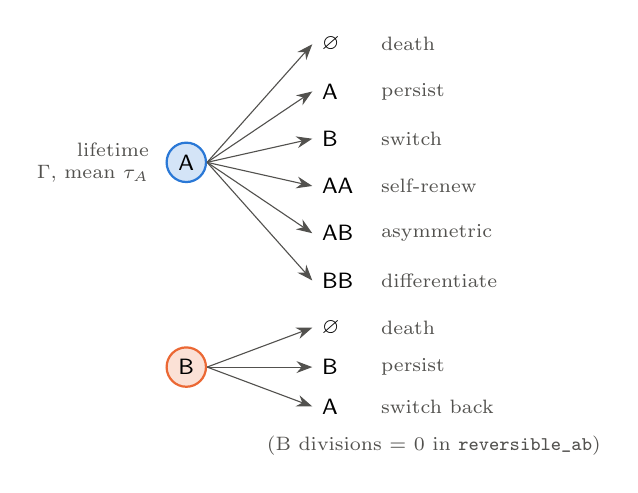
\begin{tikzpicture}[font=\footnotesize\sffamily,
  cA/.style={circle,draw=cblue,fill=cblue!20,thick,minimum size=5mm,inner sep=0},
  cB/.style={circle,draw=corange,fill=corange!20,thick,minimum size=5mm,inner sep=0},
  arr/.style={-{Stealth[length=2mm]},inkgray}]
\node[cA] (a) at (0,0) {A};
\node[font=\scriptsize,inkgray,align=right,anchor=east] at (-0.35,0) {lifetime\\$\Gamma$, mean $\tau_A$};
\foreach \y/\lab/\d [count=\i] in {1.5/death/{$\varnothing$},0.9/persist/{A},0.3/switch/{B},-0.3/self-renew/{AA},-0.9/asymmetric/{AB},-1.5/differentiate/{BB}}{
  \node[anchor=west] (o\i) at (1.6,\y) {\d};
  \node[anchor=west,inkgray,font=\scriptsize] at (2.35,\y) {\lab};
  \draw[arr] (a.east) -- (o\i.west);
}
\node[cB] (b) at (0,-2.6) {B};
\foreach \y/\lab/\d [count=\i] in {-2.1/death/{$\varnothing$},-2.6/persist/{B},-3.1/switch back/{A}}{
  \node[anchor=west] (p\i) at (1.6,\y) {\d};
  \node[anchor=west,inkgray,font=\scriptsize] at (2.35,\y) {\lab};
  \draw[arr] (b.east) -- (p\i.west);
}
\node[font=\scriptsize,inkgray,anchor=west] at (0.9,-3.6) {(B divisions = 0 in \code{reversible_ab})};
\end{tikzpicture}
\end{minipage}

\begin{table}[H]\centering\footnotesize
\caption{Reference truth $\theta^\star$ used by every experiment unless stated (\code{law.reference}); one founder cell of type A. Prior probability of exceeding the truth under the uniform Dirichlet: A$\to$AA 1.8\%; B$\to$A 0.03\% (\code{two_type}) or 4\% (\code{reversible_ab}).}\label{tab:truth}
\begin{tabular}{@{}lrrrrrrl@{}}\toprule
Type & death & persist & switch & $\to$AA & $\to$AB & $\to$BB & mean lifetime (BH) \\\midrule
A & 0.03 & 0.03 & 0.05 (A$\to$B) & \textbf{0.55} & 0.05 & 0.29 & \tA{} = 20\,h \\
B & 0.10 & 0.10 & \textbf{0.80} (B$\to$A) & 0 & 0 & 0 & \tB{} = 30\,h \\\bottomrule
\multicolumn{8}{@{}l}{BH lifetimes: Gamma, shape 8 (CV 0.35). GW: one event per generation.}
\end{tabular}
\end{table}

\subsection{Two simulators}
\begin{center}\footnotesize
\begin{tabularx}{\linewidth}{@{}P{2.5cm}YY@{}}\toprule
 & \textbf{Galton--Watson (GW)} & \textbf{Bellman--Harris (BH)} \\\midrule
Time & synchronous generations; endpoints in \emph{generations} (real-like: 6 and 10) & continuous; Gamma lifetimes per type; endpoints in \emph{hours} (real-like: 144 and 240\,h = days 6, 10) \\
Extra parameters & none & \tA, \tB{} (log-uniform prior); shape fixed (8) \\
Sampling & exact detection-conditioned sampler; exact observed fraction & forward simulation + rejection; observed fraction estimated \\
Cost & cheap & slower (rejection sampling; P0 timing not run) \\\bottomrule
\end{tabularx}
\end{center}
GW and BH share the outcome law but not the time unit; a GW generation is \emph{not} a day (X3 needs a mapping).

\subsection{Observation, data model and inference model}
\begin{itemize}
\item \textbf{Observation}: biology $\to$ capture (Binomial per true type) $\to$ labelling (confusion matrix true type $\times$ label; may be rectangular, e.g.\ hidden C read as A with prob.\ $q$) $\to$ selection of \emph{recovered} clones ($\ge 1$ detected cell). Baseline: perfect capture and typing.
\item \textbf{Data}: per endpoint, A and B counts of each recovered organoid. Endpoints are destructive: different organoids per endpoint.
\item \textbf{Misspecification}: the reference data come from a separate \emph{data model} (\code{data.simulator}, \code{data.law}, \code{data.observation}, with seed \code{data_seed}); the \emph{inference model} defines prior, training simulations and checks. An error is tested by changing one side only.
\end{itemize}

\subsection{Inference}
\begin{itemize}
\item \textbf{NPE} (\code{sbi} 0.27, neural spline flow, 5 transforms, width 64), amortised, 1 round; sequential NPE (SNPE) only in E0.
\item \textbf{Summaries} (\code{moments}): per endpoint, mean, sd, quantiles of $\log(1+n)$ for A, B, total; fraction of clones containing each type; fraction empty; correlation of log counts.
\item \textbf{Budgets}: \code{dev} = 5\,000 simulations (all BH and most GW error experiments); 20\,000 for E0/design comparison; E0 also 50\,000. E0 showed 5k$\to$50k does not change recovery. Per run: 2\,000 posterior samples, SBC on 200 prior draws, PPC with 200 datasets.
\item \textbf{Parameterisation}: stick-breaking of each simplex (exact Dirichlet reparameterisation).
\end{itemize}

\subsection{Pipeline and experiment logic}
\begin{center}
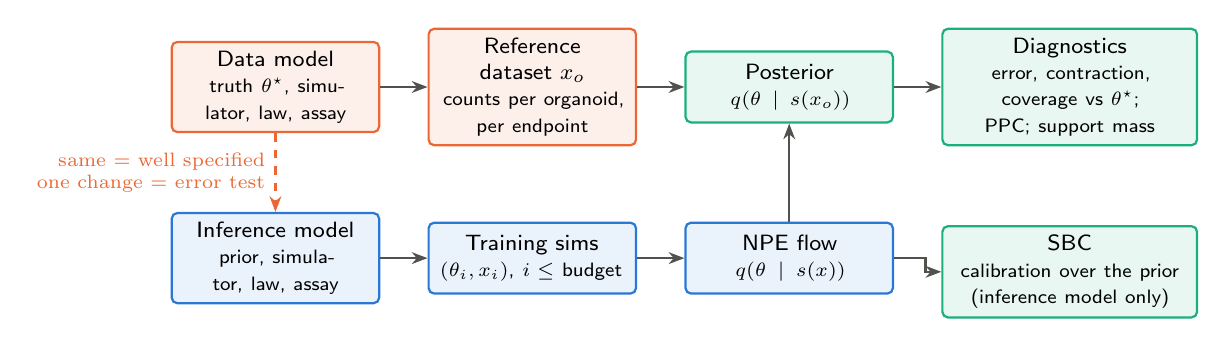
\begin{tikzpicture}[font=\footnotesize\sffamily, node distance=4mm and 6mm,
  box/.style={draw=#1,fill=#1!10,rounded corners=2pt,thick,align=center,minimum height=9mm,text width=24mm},
  box/.default=cblue,
  arr/.style={-{Stealth[length=2mm]},thick,inkgray}]
\node[box=corange] (dm) {Data model\\\scriptsize truth $\theta^\star$, simulator, law, assay};
\node[box=corange,right=of dm] (xo) {Reference dataset $x_o$\\\scriptsize counts per organoid, per endpoint};
\node[box=cblue,below=10mm of dm] (im) {Inference model\\\scriptsize prior, simulator, law, assay};
\node[box=cblue,right=of im] (sims) {Training sims\\\scriptsize $(\theta_i, x_i)$, $i\le$ budget};
\node[box=cblue,right=of sims] (npe) {NPE flow\\\scriptsize $q(\theta\mid s(x))$};
\node[box=caqua,right=of xo] (post) {Posterior\\\scriptsize $q(\theta\mid s(x_o))$};
\node[box=caqua,right=of post,text width=30mm] (diag) {Diagnostics\\\scriptsize error, contraction, coverage vs $\theta^\star$; PPC; support mass};
\node[box=caqua,below=10mm of diag,text width=30mm] (sbc) {SBC\\\scriptsize calibration over the prior (inference model only)};
\draw[arr] (dm) -- (xo);
\draw[arr] (im) -- (sims);
\draw[arr] (sims) -- (npe);
\draw[arr] (npe) -- (post);
\draw[arr] (xo) -- (post);
\draw[arr] (post) -- (diag);
\draw[arr] (npe.east) -- ++(4mm,0) |- (sbc.west);
\draw[arr,dashed,corange] (dm.south) -- node[left,font=\scriptsize,align=right]{same = well specified\\one change = error test} (im.north);
\end{tikzpicture}
\end{center}
\textbf{Experiment logic}: vary one error on the data side (or one assumption on the inference side), keep everything else at the baseline, and compare with the \emph{well-specified control of the same sweep} (same seeds, same datasets; often the same trained network, so differences are paired by seed).

\subsection{Diagnostics and how to read them}
\begin{center}\footnotesize
\begin{tabularx}{\linewidth}{@{}P{3.0cm}YY@{}}\toprule
\textbf{Metric} & \textbf{Definition} & \textbf{How to read} \\\midrule
Posterior mean / error & mean of 2\,000 posterior samples; $|$mean $-$ truth$|$. MAE over probabilities only (\code{mae_probabilities}); lifetimes separately & compare misspecified vs control; ``shift'' = difference of posterior means, paired by seed, $\pm$ paired SE over 5 seeds \\
Contraction & $1-\mathrm{Var}_\text{post}/\mathrm{Var}_\text{prior}$ & 0 = data uninformative; $<0$ = wider than prior; $>0.5$ = informative \\
90\% coverage across seeds & number of seeds (of 5) whose 90\% credible interval contains the truth & 4--5/5 expected; 0/5 with high contraction = confident bias \\
SBC coverage error & mean $|$empirical $-$ nominal$|$ coverage of central intervals (50--95\%) over 200 prior draws & $\le 0.03$ = calibrated. Averages over the prior: blind to tail truths and to misspecification \\
PPC fraction outside 95\% & share of summary features whose observed value lies outside the 95\% posterior predictive interval & well specified: 0--0.03. Higher = the model cannot reproduce the data. Relative check \\
Posterior support mass & share of the NPE posterior inside the prior support & well specified $\approx$\,0.5--0.9 (not 1). $\approx 0$ = model cannot explain the data; few/no samples, not an estimate \\
Recovered (TODO criterion) & contraction $>0.5$, $|$error$|<0.05$, coverage $\ge 4/5$ & used for ``organoids needed'' (E4) \\\bottomrule
\end{tabularx}
\end{center}

\begin{keybox}
\textbf{Reading rules used throughout.}
(1) \emph{BH baseline bias}: well-specified BH runs give A$\to$AA $\approx$ 0.32 and \tA{} $\approx$ 16\,h (truth 0.55, 20\,h); BH misspecified arms are compared with their control, never with the truth.
(2) With all transitions free, B's row is prior-dominated (E0).
(3) A misspecification that raises neither PPC nor lowers support mass is \emph{undetectable from the fit}.
(4) 5 seeds per setting: effects below $\approx$\,2 paired SE are not resolved.
(5) Wall times in run metrics were measured under heavy contention; only the device benchmark (\S\ref{sec:gpu}) measures speed.
\end{keybox}

% ====================================================================== PART I
\clearpage
\part{Identifiability and the role of the prior}\label{part:ident}
\partintro{\textbf{Motivation.} Every later question (how many organoids, which errors matter) presupposes that the parameters can be learned from endpoint counts at all. The very first fits failed on one parameter, B$\to$A. This part establishes why: whether the prior or the model is at fault decides what the remedy is (a different prior, more data, or a biological constraint). It ends with the constraint that all later experiments adopt (B divisions = 0, \code{reversible_ab}).}

% ---------------------------------------------------------------------- E0
\expsec{E0 --- Identifiability of B's row (GW)}{sec:e0}
\Why{This is the starting point. With the general two-type law (all 12 outcomes free) the first well-specified fits returned B$\to$A $\approx 0.2$ for a truth of 0.8. Nothing downstream can be interpreted until this is understood.}
\Q
With all transitions free, B$\to$A (true 0.80) came out at $\approx$\,0.2. Is this under-training, one bad dataset, miscalibration, a prior-tail effect, or non-identifiability (switching vs division)?
\Setup
\begin{setup}
Simulator & Galton--Watson, perfect observation \\
Law (free) & \code{two_type} (10) vs \code{reversible_ab} (7; B divisions fixed to their true 0) \\
Data vs inference & well specified (same $\theta^\star$, Table~\ref{tab:truth}) \\
Design & generations 4, 8, 12 $\times$ 32 clones (96 organoids) \\
Inference / budget & NPE amortised 5k, 20k, 50k; SNPE 4 rounds $\times$ 5k; \code{two_type} with flat prior on B$\to$A (Beta(1,1)), 20k \\
Seeds / runs & 5 / 40 (+ direct checks: C2ST of mean-preserving alternatives, 500 datasets per side) \\
Varied & law, budget, method, prior \\
Folder & \res{results/b_row/} (\res{distinguish.csv}, \res{truth_vs_posterior_20k*.csv}) \\
\end{setup}
\Result
\figorpending{e0_bto_a}{1.0}{B$\to$A posterior mean $\pm$ sd per seed. Orange: all B outcomes free (uniform Dirichlet; squares: SNPE). Green: flat prior on B$\to$A. Blue: B divisions fixed to 0.}{E0 figure.}
\begin{center}\footnotesize
\begin{tabular}{@{}llrrrrr@{}}\toprule
Law & Training & B$\to$A mean & post.\ sd & contraction & covered & MAE (all) \\\midrule
\code{two_type} & 5k / 20k / 50k & 0.20 / 0.21 / 0.22 & 0.14--0.15 & $-0.03$ / $-0.13$ / $-0.18$ & 0/15 & 0.14 \\
\code{two_type} & SNPE 4$\times$5k & 0.21 & 0.16 & $-0.22$ & 0/5 & 0.14 \\
\code{two_type}, flat prior & 20k & 0.53 & 0.21 & 0.46 & 4/5 & 0.10 \\
\code{reversible_ab} & 5k / 20k / 50k & 0.72 / 0.71 / 0.70 & 0.13--0.14 & 0.67 / 0.71 / 0.69 & 15/15 & 0.05 \\\bottomrule
\end{tabular}
\end{center}
\begin{minipage}[c]{0.46\linewidth}
\figorpending{e0_c2st}{1.0}{C2ST accuracy separating the truth from a mean-preserving alternative (B$\to$AA $=a$, B$\to$A $=0.8-2a$, B death $=0.1+a$). 0.5 = indistinguishable.}{C2ST heat map.}
\end{minipage}\hfill
\begin{minipage}[c]{0.5\linewidth}\footnotesize
\begin{itemize}
\item SBC coverage error 0.02--0.04 in every arm (looks calibrated).
\item PPC $\le 0.014$ in every arm.
\item Flat prior: corr(B$\to$A, B$\to$AA) $= -0.67$; SBC fails (0.069) for B's other coordinates (concentration 0.2), not for B$\to$A.
\item Truth-vs-posterior C2ST: inconclusive (0.62--0.95 in both laws).
\end{itemize}
\end{minipage}
\Comment
\begin{itemize}
\item Under-training, dataset and calibration are ruled out: 10$\times$ more simulations, 5 datasets, SBC all unchanged.
\item Main cause = prior tail: B$\to$A $\sim$ Beta(1,5), P($>0.8$) = 0.03\% ($\approx$\,15 of 50k training simulations). SNPE cannot help: round 0 is already prior-like. \emph{Revised by X5 (\S\ref{sec:x5a}, \S\ref{sec:x5c})}: with B divisions free B$\to$A is not recovered at any truth $\ge 0.5$ (bulk included) nor with 1024 organoids, so the confounding below is the root cause and the tail only makes it visible.
\item Data weakly confound switching with division: even with a flat prior the posterior is wide (sd 0.21) and anti-correlated with B$\to$AA. They differ only in clone-size variability; 128--512 clones/endpoint make moderate differences detectable.
\item Consequence: fix what biology allows (B divisions = 0 $\Rightarrow$ B$\to$A $\approx$ 0.70, contraction 0.7); otherwise report prior sensitivity. All later experiments use \code{reversible_ab}.
\end{itemize}
\Leads{Two explanations remain open: the prior tail (B$\to$A = 0.8 has 0.03\% prior mass) and structural confounding of switching with division (the flat-prior posterior is wide and anti-correlated with B$\to$AA). X5a (\sref{sec:x5a}) separates them by moving the truth through the prior; X5c (\sref{sec:x5c}) asks whether more organoids, which the C2ST suggests would help, can overrule the prior.}

% ---------------------------------------------------------------------- X5a
\expsec{X5a --- Role of the prior I: truth position $\times$ prior shape (GW)}{sec:x5a}\label{sec:x5}
\Why{E0 (\sref{sec:e0}) attributed the B-row failure mainly to the prior tail, with weak confounding as a second cause. If the tail were the cause, a truth in the prior bulk or a flatter prior should be recovered; if the confounding were the cause, no truth position or prior should help unless B divisions are fixed.}
\textbf{About X5.} X5 (``role of the prior'') is one experiment in four parts, placed here where each is motivated: X5a (this section), X5c (\sref{sec:x5c}), X5d (\sref{sec:x5d}), X5b (\sref{sec:x5b}). Common to all: synthetic data, real-like design (GW generations 6/10 or BH 144/240\,h; 165/101 clones unless swept), perfect observation, one A founder, NPE 5k (\code{budget=dev}), SBC 200, PPC 200; 355 runs in total (X5a 250, X5b 15, X5c 30, X5d 60). Folder \res{results/x5/} (overview \res{info.md}, per-part tables \res{x5*_findings.md}).
\Q Does recovery of B$\to$A depend on where the truth sits in the prior (0.1--0.9) and on the prior's shape, with B divisions free vs fixed? Is E0's failure a tail-truth effect?
\Setup
\begin{setup}
Data model & GW; B$\to$A $\in \{0.1, 0.3, 0.5, 0.7, 0.9\}$, B death = B persist = $(1-\text{B}\to\text{A})/2$; other parameters $\theta^\star$ \\
Laws (data = inference) & \code{two_type} (B divisions free, 10 free) and \code{reversible_ab} (B divisions fixed to 0, 7 free). Prior P(B$\to$A $>0.9$): $10^{-5}$ resp.\ 0.01 \\
Priors (inference only) & uniform Dirichlet; Jeffreys (all concentrations 0.5); flat marginal on B$\to$A (Beta(1,1): concentration 0.2 on B's 5 other outcomes in \code{two_type}, 0.5 on death/persist in \code{reversible_ab}). \emph{Biological} (Dirichlet pseudo-counts per type, each row sums to 1; total $\approx$\,5--6 = weakly informative): \textbf{bio-B} = B row only, death/persist/to\_A 1.5 and B divisions 0.2 each (\code{two_type}; fixed in \code{reversible_ab}), A row uniform; \textbf{bio} = bio-B plus A row death/persist/to\_B 0.5, div\_AA 2, div\_AB 1, div\_BB 1.5. Rationale: encode the biology without the answer --- A (stem-like) mostly divides, self-renewal most likely; B (differentiated) rarely divides but may die, persist or switch back. bio-B vs bio separates B's prior from A's \\
Seeds / runs & 5 / 125 per law (250: 150 reference + 100 biological) \\
Folder & \res{results/x5/a_two_type/}, \res{results/x5/a_reversible_ab/}, biological priors in \res{a_two_type_bio/}, \res{a_reversible_ab_bio/} (pooled \res{x5a_groups.csv}, \res{x5a_runs.csv} in the first two) \\
\end{setup}
\Result
\figorpending{x5a}{0.9}{X5a: B$\to$A posterior mean (mean over 5 seeds) $\pm$ mean posterior sd against the true B$\to$A, one line per prior (slightly offset). Top: reference priors; bottom: biological priors bio-B and bio, with the uniform and flat-B$\to$A means as thin reference lines. Dashed: identity (perfect recovery). Dotted: uniform-prior mean (1/6 left, 1/3 right).}{X5a figure.}
\begin{center}\footnotesize
\begin{tabular}{@{}rllllll@{}}\toprule
 & \multicolumn{3}{c}{B divisions free (\code{two_type})} & \multicolumn{3}{c}{B divisions fixed (\code{reversible_ab})} \\\cmidrule(lr){2-4}\cmidrule(l){5-7}
Truth & uniform & Jeffreys & flat B$\to$A & uniform & Jeffreys & flat B$\to$A \\\midrule
0.1 & 0.04 (3/5) & 0.04 (5/5) & 0.12 (5/5) & 0.15 (5/5) & 0.16 (4/5) & 0.17 (5/5) \\
0.3 & 0.11 (1/5) & 0.11 (2/5) & 0.23 (5/5) & 0.37 (5/5) & 0.42 (5/5) & 0.43 (4/5) \\
0.5 & 0.13 (0/5) & 0.12 (0/5) & 0.23 (2/5) & 0.44 (5/5) & 0.45 (5/5) & 0.49 (5/5) \\
0.7 & 0.18 (0/5) & 0.20 (0/5) & 0.36 (3/5) & 0.67 (5/5) & 0.70 (5/5) & 0.74 (5/5) \\
0.9 & 0.22 (0/5) & 0.26 (0/5) & 0.54 (1/5) & 0.79 (5/5) & 0.80 (5/5) & 0.85 (5/5) \\\midrule
SBC error & 0.037 & 0.054 & 0.080 & 0.032 & 0.056 & 0.037 \\\bottomrule
\end{tabular}

\medskip
\begin{tabular}{@{}rllll@{}}\toprule
 & \multicolumn{2}{c}{B divisions free (\code{two_type})} & \multicolumn{2}{c}{B divisions fixed (\code{reversible_ab})} \\\cmidrule(lr){2-3}\cmidrule(l){4-5}
Truth & bio-B & bio (A+B) & bio-B & bio (A+B) \\\midrule
0.1 & 0.10 (5/5) & 0.09 (5/5) & 0.16 (4/5) & 0.14 (5/5) \\
0.3 & 0.24 (5/5) & 0.25 (5/5) & 0.37 (4/5) & 0.33 (5/5) \\
0.5 & 0.26 (1/5) & 0.28 (1/5) & 0.42 (5/5) & 0.38 (4/5) \\
0.7 & 0.40 (2/5) & 0.47 (3/5) & 0.63 (5/5) & 0.61 (4/5) \\
0.9 & 0.54 (1/5) & 0.59 (1/5) & 0.73 (1/5) & 0.75 (3/5) \\\midrule
run MAE & 0.05--0.09 & 0.03--0.07 & 0.03--0.06 & 0.03--0.05 \\
SBC error & 0.052 & 0.055 & 0.033 & 0.041 \\
B-division mass & 0.21 & 0.11 & --- & --- \\\bottomrule
\end{tabular}

B$\to$A posterior mean (seeds covered by the 90\% interval). Run MAE = range over truths of the mean per-run MAE (all free parameters); B-division mass = posterior total of B$\to$AA/AB/BB (truth 0; 0.54 under the uniform and flat priors). Reference priors, run MAE: free 0.12--0.15 (uniform), 0.10--0.16 (flat); fixed 0.02--0.06 (uniform). Numbers: \res{tables/x5a.csv}.
\end{center}
\Comment
\begin{itemize}
\item \textbf{B divisions free: the estimate hardly follows the truth} (0.04 $\to$ 0.22 as the truth goes 0.1 $\to$ 0.9, uniform prior); no truth $\ge 0.5$ is covered under the uniform or Jeffreys prior, and B$\to$A contraction falls to $\le 0$ at 0.9. The data cannot separate switching from division, so the prior sets the answer --- at \emph{every} truth position, not only in the tail.
\item A flat prior on B$\to$A tracks better (0.12 $\to$ 0.54) but still shrinks heavily and costs calibration (SBC 0.080) and coverage of the other parameters (run coverage 0.62--0.87).
\item \textbf{B divisions fixed: every truth is recovered under every prior} (B$\to$A contraction 0.73--0.94; the three priors differ by $\le 0.06$, mild shrinkage at the extremes). The prior only matters once the model is structurally confounded.
\item Conclusion for E0 (\S\ref{sec:e0}): the B-row failure is structural (switching vs division), not a bad truth position; a prior cannot substitute for the constraint.
\item \textbf{Biological priors.} \emph{B divisions free}: the soft ``B rarely divides'' prior cuts the posterior B-division mass from 0.54 to 0.21 (bio-B) and 0.11 (bio); B$\to$A tracks like the flat prior (0.54--0.59 at truth 0.9) but with better calibration (SBC 0.05 vs 0.08) and the lowest error of any free-B prior (run MAE 0.03--0.07 for bio; the A-row prior gives most of this gain). It is still far from the hard constraint (0.79, 5/5 at truth 0.9): truths $\ge 0.5$ are mostly not covered. \emph{B divisions fixed}: the symmetric 1.5 prior on B's three outcomes (mean 1/3) shrinks B$\to$A toward 1/3, and truth 0.9 is covered in only 1/5 (bio-B) and 3/5 (bio) seeds; the A-row prior lowers the error and raises support mass (0.79--0.89 vs 0.64--0.79 uniform). A soft biological prior helps but does not replace the constraint; with the constraint, keep B's prior near-uniform.
\end{itemize}
\Leads{The constraint, not the prior, decides. Remaining question: is it only a matter of sample size? (X5c, \sref{sec:x5c}).}

% ---------------------------------------------------------------------- X5c
\expsec{X5c --- Role of the prior II: data vs prior at a tail truth (GW)}{sec:x5c}
\Why{X5a (\sref{sec:x5a}) showed the confounding at the real-like size (165/101 clones). E0's C2ST (\sref{sec:e0}) predicted that 128--512 clones per endpoint make moderate switching/division differences detectable, so a large enough experiment might overrule the prior without a constraint.}
\Q With all transitions free and a tail truth (B$\to$A = 0.9, prior P $=10^{-5}$ under Beta(1,5)), how many organoids overrule the prior?
\Setup
\begin{setup}
Data model & GW, \code{two_type}; B: death 0.05, persist 0.05, B$\to$A 0.9 (B divisions 0); A row $\theta^\star$ \\
Inference & \code{two_type} (10 free), uniform Dirichlet vs flat marginal on B$\to$A (concentration 0.2 on B's other outcomes) \\
Design & generations 6/10 $\times$ \{32, 128, 512\} clones per endpoint \\
Seeds / runs & 5 / 30 \\
Folder & \res{results/x5/c_data_vs_prior/} (\res{x5c_groups.csv}, \res{x5c_runs.csv}) \\
\end{setup}
\Result
\figorpending{x5c}{0.72}{X5c: B$\to$A (mean over 5 seeds $\pm$ mean posterior sd) and B$\to$AA posterior mean against clones per endpoint; dashed = truth.}{X5c figure.}
\begin{center}\footnotesize
\begin{tabular}{@{}lrrrrrrrrr@{}}\toprule
Prior & clones & B$\to$A (0.9) & post.\ sd & cov. & contr. & B$\to$AA (0) & MAE & support & SBC \\\midrule
uniform & 32 & 0.19 & 0.14 & 0/5 & 0.01 & 0.31 & 0.161 & 0.79 & 0.031 \\
 & 128 & 0.21 & 0.15 & 0/5 & $-0.10$ & 0.32 & 0.151 & 0.72 & 0.037 \\
 & 512 & 0.25 & 0.15 & 0/5 & $-0.17$ & 0.29 & 0.139 & 0.55 & 0.044 \\
flat B$\to$A & 32 & 0.47 & 0.22 & 2/5 & 0.44 & 0.28 & 0.119 & 0.49 & 0.078 \\
 & 128 & 0.55 & 0.19 & 1/5 & 0.57 & 0.26 & 0.101 & 0.42 & 0.081 \\
 & 512 & 0.59 & 0.17 & 1/5 & 0.65 & 0.23 & 0.086 & 0.46 & 0.083 \\\bottomrule
\end{tabular}
\end{center}
PPC $\le 0.03$ in every group. Numbers: \res{tables/x5c.csv}.
\Comment
\begin{itemize}
\item \textbf{1024 organoids do not overrule the uniform prior}: B$\to$A moves 0.19 $\to$ 0.25 (truth 0.9), never covered, contraction $\le 0$; the mass goes to B$\to$AA ($\approx$\,0.3, truth 0) --- the switching/division confounding of E0.
\item A flat prior helps and improves with data (0.47 $\to$ 0.59, contraction up to 0.65) but is still far from 0.9 at 1024 organoids and costs calibration (SBC 0.08).
\item Endpoint counts of this kind cannot resolve the confounding by sample size at realistic scales; the structural constraint (B divisions fixed, X5a) is what works.
\end{itemize}
\Leads{Part~\ref{part:design}: with B divisions fixed (\code{reversible_ab}) as the baseline, which design and how many organoids? The design comparison (\sref{sec:design}) also re-checks the free law at up to 384 organoids.}

% ====================================================================== PART II
\clearpage
\part{Design and amount of data}\label{part:design}
\partintro{\textbf{Motivation.} With an identifiable model (Part~\ref{part:ident}), the planning question is the design: which days to measure and how many organoids per day. E0 showed that the information lies in clone-size variability across time, which suggests that the number of endpoints may matter as much as the number of organoids. We first compare one and three endpoints in GW, then map the full grid in GW and BH. The BH half produces the result that drives Part~\ref{part:timing}.}

% ---------------------------------------------------------------------- design
\expsec{Design comparison --- one vs three endpoints (GW)}{sec:design}
\Why{Part~\ref{part:ident} fixed the law (B divisions = 0, \sref{sec:x5a}). E0 used 3 endpoints $\times$ 32 clones; the real data have 2 endpoints, and a wet-lab plan can trade endpoints for organoids. Which matters more, at equal total organoids?}
\Q Which planned design identifies the model best, and is it the number of time points or the number of organoids that matters?
\Setup
\begin{setup}
Simulator & Galton--Watson, perfect observation \\
Law (free) & \code{two_type} (10) and \code{reversible_ab} (7) \\
Data vs inference & well specified, $\theta^\star$ \\
Design & \code{single_128}: gen.\ 12 $\times$ 128; \code{three_128}: gen.\ 4, 8, 12 $\times$ 128; \code{single_384}: gen.\ 12 $\times$ 384; reference \code{three_32} (from E0) \\
Inference / budget & NPE amortised, 20k \\
Seeds / runs & 5 / 30 (+ 10 reference runs from E0) \\
Varied & design $\times$ law \\
Folder & \res{results/design_comparison/} \\
\end{setup}
\Result
\figorpending{design_comparison}{1.0}{Left, centre: MAE and mean contraction per design (mean $\pm$ sd over 5 seeds); total organoids in brackets. Right: contraction per parameter, B divisions fixed.}{Design figure.}
\begin{center}\footnotesize
\begin{tabular}{@{}lrrrrrrr@{}}\toprule
Design (\code{reversible_ab}) & organoids & MAE & contraction & 90\% cov. & B$\to$A & B$\to$A contr. & PPC \\\midrule
1 $\times$ 128 & 128 & 0.079 & 0.77 & 0.87 & 0.61 $\pm$ 0.17 & 0.50 & 0.000 \\
3 $\times$ 32 & 96 & 0.052 & 0.86 & 0.96 & 0.71 $\pm$ 0.13 & 0.71 & 0.008 \\
1 $\times$ 384 & 384 & 0.058 & 0.84 & 0.93 & 0.67 $\pm$ 0.12 & 0.72 & 0.000 \\
\textbf{3 $\times$ 128} & 384 & \textbf{0.028} & \textbf{0.93} & 0.93 & \textbf{0.78 $\pm$ 0.09} & \textbf{0.87} & 0.031 \\\midrule
\code{two_type}, any design & 96--384 & 0.13--0.15 & 0.45--0.53 & 0.69--0.78 & 0.18--0.25 & $\le -0.03$ & $\le$ 0.014 \\\bottomrule
\end{tabular}
\end{center}
\Comment
\begin{itemize}
\item At equal organoids, 3 endpoints halve the error of 1 (0.028 vs 0.058). Gains are in dynamics: A$\to$AB contraction 0.90 vs 0.60, B$\to$A 0.87 vs 0.72.
\item 96 organoids over 3 endpoints $\approx$ 384 at one endpoint.
\item With all transitions free no design recovers B's row (B$\to$A contraction $\le 0$) --- consistent with E0.
\item Calibration fine everywhere (SBC 0.02--0.03). Caveat: GW, one truth, generations not days.
\end{itemize}
\Leads{One slice (GW, generations 4/8/12, 20k simulations). E4 maps the full grid of organoids $\times$ endpoint sets, including the real-like \{6, 10\}: GW first (\sref{sec:e4gw}), then BH (\sref{sec:e4}).}

% ---------------------------------------------------------------------- E4 GW
\expsec{E4 --- Amount of data: organoids and endpoints (GW)}{sec:e4gw}
\Why{The design comparison (\sref{sec:design}) showed that three endpoints beat one at equal organoids. For a plan we need the minimum number of organoids per endpoint for each parameter and the best endpoint set, systematically. GW comes first: it has no lifetimes, so it shows what endpoint counts can deliver when the time scale is known.}
\Q How do contraction and error depend on organoids per endpoint (16--512) and on the measured generations? What is the minimum number to recover each parameter when there is no lifetime ridge?
\Setup
\begin{setup}
Simulator & Galton--Watson (endpoints in \emph{generations}; day-mapping nominal) \\
Law (free) & \code{reversible_ab} (7 probabilities) \\
Data vs inference & well specified, $\theta^\star$ \\
Design & clones per endpoint $\in \{16,\dots,512\}$ $\times$ generations \{10\}, \{6,10\}, \{6,10,14\}, \{4,6,10\} \\
Inference / budget & NPE amortised, 5k \\
Seeds / runs & 5 / 120 (all with 2\,000 posterior samples, 200 SBC cases) \\
Folder & \res{results/e4/gw/} \\
\end{setup}
\Result
\figorpending{e4_gw_heat}{1.0}{E4 GW: mean contraction and MAE of the outcome probabilities (mean over 5 seeds); endpoints in generations.}{E4 GW heat map.}
\figorpending{e4_gw_params}{1.0}{E4 GW: posterior means (mean $\pm$ SE over seeds) vs organoids per endpoint; dashed = truth.}{E4 GW parameter lines.}
\begin{center}\footnotesize
\textbf{Minimum organoids per endpoint for ``recovered''} (contraction $>0.5$, $|$error$|<0.05$, $\ge$\,4/5 covered; must hold at every larger size; --- = not reached; for BH see \S\ref{sec:e4})\\[2pt]
\begin{tabular}{@{}lrrrr@{}}\toprule
 & \multicolumn{4}{c}{\textbf{GW}, generations} \\
Parameter & \{10\} & \{6, 10\} & \{6, 10, 14\} & \{4, 6, 10\} \\\midrule
A death, A persist, A$\to$B & 16 & 16 & 16 & 16 \\
B death & 32 & 16 & 16 & 16 \\
A$\to$AA & 256 & 16 & 16 & ---$^a$ \\
A$\to$BB & --- & 256 & --- & \textbf{32} \\
B persist & --- & 512 & --- & \textbf{64} \\
B$\to$A & --- & --- & --- & \textbf{128} \\
A$\to$AB & --- & 512 & --- & 512 \\\bottomrule
\multicolumn{5}{@{}l}{$^a$ error $\le 0.04$ at every size, but coverage 2--4/5 (narrow posteriors, sd $\approx$ 0.02).}
\end{tabular}
\end{center}
\Comment
\begin{itemize}
\item \textbf{Design ranking}: an early endpoint is worth most (\{4,6,10\} best at every size); a late extra endpoint (\{6,10,14\}) adds little over \{6,10\}; one endpoint plateaus and cannot separate A$\to$AB from A$\to$BB (0.15--0.24 vs 0.05; 0.15--0.20 vs 0.29) at any size.
\item \textbf{Without lifetimes everything is recoverable}: with \{4,6,10\} and $\approx$\,128 organoids per endpoint all probabilities except A$\to$AB (512) meet the criterion; A$\to$AA is right from 16 organoids. The GW numbers are the attainable target \emph{if} division times are known (BH with lifetimes fixed: MAE 0.059, \S\ref{sec:ridge}).
\item Checks: single well-specified GW runs reach PPC 0.10 and support mass 0.07 (\{4,6,10\}, seed 4): borderline single values are not evidence of misspecification.
\item Caveat: generations are not days; one truth, perfect assay, single A founders, 5k simulations. Planned extension (not run): \code{law=two_type} at 256--512 clones.
\end{itemize}
\Leads{The same grid in BH (\sref{sec:e4}), the simulator closer to the real data (time in hours, free lifetimes). Does the ranking survive, and are the GW numbers reached?}

% ---------------------------------------------------------------------- E4 BH
\expsec{E4 --- Amount of data: organoids and endpoints (BH), and comparison with GW}{sec:e4}
\Why{GW (\sref{sec:e4gw}) recovers every probability by $\approx$\,128 organoids with \{4,6,10\}. BH adds two free lifetimes and measures time in days; it is the model that will be fitted to real data.}
\Q As \S\ref{sec:e4gw} for Bellman--Harris (endpoints in hours): how do contraction and error depend on organoids per endpoint (16--512) and on the measured days? What is the minimum number to recover each parameter, and are the GW numbers reached?
\Setup
\begin{setup}
Simulator & Bellman--Harris, Gamma lifetimes shape 8 \\
Law (free) & \code{reversible_ab}: 7 probabilities + \tA, \tB{} (9) \\
Data vs inference & well specified, $\theta^\star$ \\
Design & clones per endpoint $\in \{16,32,64,128,256,512\}$ $\times$ endpoints \{240\}, \{144, 240\}, \{144, 240, 336\}, \{96, 144, 240\}\,h = days \{10\}, \{6,10\}, \{6,10,14\}, \{4,6,10\} \\
Inference / budget & NPE amortised, 5k \\
Seeds / runs & 5 / 120 \\
Varied & clones $\times$ endpoint set \\
Folder & \res{results/e4/bh/} \\
\end{setup}
\Result
\figorpending{e4_bh_heat}{1.0}{Mean contraction and MAE of the 7 outcome probabilities (mean over 5 seeds).}{E4 BH heat map.}
\figorpending{e4_bh_params}{1.0}{Posterior means (mean $\pm$ SE over seeds) vs organoids per endpoint, one line per endpoint set; dashed = truth.}{E4 BH parameter lines.}
\begin{center}\footnotesize
\textbf{Minimum organoids per endpoint for ``recovered''} (contraction $>0.5$, $|$error$|<0.05$, $\ge$\,4/5 covered); --- = not reached at 512.\\[2pt]
\begin{tabular}{@{}lrrrr@{}}\toprule
Parameter & day 10 & days 6, 10 & days 6, 10, 14 & days 4, 6, 10 \\\midrule
A death, A$\to$B (small truths) & 16 & 16 & 16 & 16 \\
A$\to$BB & --- & 512 & 256 & \textbf{128} \\
B death & --- & 256 & 256 & \textbf{128} \\
A$\to$AB & --- & --- & --- & \textbf{256} \\
A$\to$AA, A persist, B persist, B$\to$A & --- & --- & --- & --- \\
\tA, \tB{} (biased: \tA{} 15--17\,h, 0/5 covered) & --- & --- & --- & --- \\\bottomrule
\end{tabular}

\medskip\textbf{Comparison with GW} (\S\ref{sec:e4gw}; same grid, endpoints in generations)\\[2pt]
\begin{tabular}{@{}lll@{}}\toprule
 & \textbf{BH} (days) & \textbf{GW} (generations) \\\midrule
Contraction, 16 $\to$ 512, \{4,6,10\} & 0.50 $\to$ 0.79 & 0.80 $\to$ 0.95 \\
MAE, 16 $\to$ 512, \{4,6,10\} & 0.114 $\to$ 0.060 & 0.052 $\to$ 0.023 \\
Single late endpoint, contraction & 0.37 $\to$ 0.50 & 0.63 $\to$ 0.85 (A$\to$AB / A$\to$BB confounded) \\
A$\to$AA (0.55) & 0.29--0.39, 0--2/5 covered & 0.47--0.54 at every design \\
B$\to$A (0.80), \{4,6,10\}, 128 / 512 & 0.65 / 0.73 & 0.78 / 0.80 \\
Support mass / PPC (well specified, per run) & 0.52--0.92 / $\le 0.042$ & 0.07--0.89 / $\le 0.10$ (group means $\le 0.021$) \\\bottomrule
\end{tabular}
\end{center}
\Comment
\begin{itemize}
\item \textbf{Same design ranking as GW} (\S\ref{sec:e4gw}): the ranking is a property of the endpoint information, not of the time model. An early endpoint (day 4) helps most; day 10 alone plateaus (contraction 0.37 $\to$ 0.50 from 16 to 512).
\item With several endpoints more organoids keep helping (MAE 0.114 $\to$ 0.060 for days 4/6/10); B$\to$A rises 0.59 $\to$ 0.73.
\item A$\to$AA (0.29--0.39) and \tA{} (15--17\,h) are never recovered; coverage falls to 0 as posteriors narrow on the wrong values: the ridge (\S\ref{sec:ridge}), not lack of data.
\item ``Recovered'' for A death / A$\to$B is easy because the truths are small ($|$error$|<0.05$ is loose there).
\item GW, without lifetimes, reaches contraction 0.80 $\to$ 0.95 and recovers A$\to$AA at every design (table above).
\item Caveat: one truth, perfect assay, single A founders, 5k simulations.
\end{itemize}
\Leads{A$\to$AA and \tA{} are wrong at \emph{every} size and endpoint set, with coverage falling as data grow: a bias, not a lack of data. Part~\ref{part:timing} opens with the hypothesis that explains it (\sref{sec:ridge}).}

% ====================================================================== PART III
\clearpage
\part{Bellman--Harris timing: the lifetime ridge}\label{part:timing}
\partintro{\textbf{Motivation.} E4 BH (\sref{sec:e4}) left a bias that more organoids do not remove. This part identifies it as a ridge (\sref{sec:ridge}), asks whether it is a property of the hand-picked truth (X5d), and tests the remedy suggested by the ridge, lifetime information, in its soft (literature prior, X5b) and hard (fixed lifetimes, E3a) form. Fixing lifetimes rests on timing assumptions: one value per type (E3a), the lifetime variability (E3b), and the absence of quiescence (E3c), which are tested last.}

% ---------------------------------------------------------------------- ridge
\expsec{BH ridge --- lifetime vs self-renewal}{sec:ridge}
\Why{E4 BH (\sref{sec:e4}): A$\to$AA 0.29--0.39 and \tA{} 15--17\,h at every design, 0/5 covered, whereas GW recovers A$\to$AA at every design (\sref{sec:e4gw}). The only structural difference is the free time scale. Hypothesis: endpoint counts fix the growth rate, which faster cycles or more self-renewal produce equally.}
\Q Is the BH baseline bias (A$\to$AA $\approx$ 0.32, \tA{} $\approx$ 16\,h) a ridge on which endpoint counts fix only a combination of lifetime and self-renewal, with the prior picking the point?
\Setup
\begin{setup}
Simulator & Bellman--Harris, shape 8 \\
Law (free) & control: \code{reversible_ab} (9); lifetimes fixed: 7; flat prior: 9 \\
Data vs inference & data always $\theta^\star$; only the inference model changes \\
Design & real-like: 144/240\,h $\times$ 165/101 \\
Inference / budget & NPE amortised, 5k \\
Arms & control (from E3b, shape 8); \tA=20, \tB=30\,h fixed; flat prior on A$\to$AA (concentration 1 vs 0.2 for A's other outcomes: A$\to$AA $\sim$ Beta(1,1)) \\
Seeds / runs & 5 / 10 (+5 control) \\
Folder & \res{results/bh_ridge/} (control: \res{results/e3b/*lifetime_shape=8*}) \\
\end{setup}
\Result
\figorpending{bh_ridge}{1.0}{(a) A$\to$AA posterior pooled over 5 seeds; dotted: uniform-Dirichlet prior Beta(1,5). (b) Joint posterior of A$\to$AA and \tA{} (blue: control; green: flat prior); star = truth. (c) Per-seed means $\pm$ sd; dashed = truth.}{Ridge figure.}
\begin{center}\footnotesize
\begin{tabular}{@{}lccc@{}}\toprule
 & Control & Lifetimes fixed & Flat prior \\\midrule
A$\to$AA (0.55) & 0.32 $\pm$ 0.10, 0/5, contr.\ 0.52 & \textbf{0.51 $\pm$ 0.04, 5/5, 0.93} & 0.46 $\pm$ 0.12, 5/5, 0.83 \\
A$\to$AB (0.05) & 0.23, 3/5 & 0.17, 2/5 & 0.20, 5/5, contr.\ 0.00 \\
B$\to$A (0.80) & 0.63, 5/5 & 0.68, 5/5 & 0.46, 3/5 \\
\tA{} (20\,h) & 15.9 $\pm$ 1.9, 0/5 & fixed & 18.9 $\pm$ 2.2, 5/5 \\
MAE (probabilities) & 0.109 & \textbf{0.059} & 0.117 \\
SBC error / PPC / support & 0.025 / 0.008 / n/r & 0.031 / 0.025 / 0.65 & 0.079 / 0.000 / 0.51 \\\bottomrule
\end{tabular}
\end{center}
\Comment
\begin{itemize}
\item Ridge confirmed: posterior corr(A$\to$AA, \tA) $\approx +0.7$ (E3c). Removing the lifetime degree of freedom recovers self-renewal and halves the error.
\item The prior chose the point: only 1.8\% of uniform-Dirichlet mass lies above 0.55. A flat prior re-centres (5/5 covered) but stays wide, degrades B$\to$A and calibration: not a fix.
\item GW has no lifetimes and no ridge: the GW control at the same design gives A$\to$AA 0.52 (\S\ref{sec:e1a}), and 0.47--0.54 at every E4 design (\S\ref{sec:e4gw}).
\item Consequence: measure A's division time (live imaging) or use it as an informative prior; otherwise report BH results with prior sensitivity. X5 tested both: a right $\pm 25\%$ lifetime prior gives A$\to$AA 0.46, MAE 0.068 (\S\ref{sec:x5b}); averaged over prior-drawn truths A$\to$AA is learned well (contraction 0.82, \S\ref{sec:x5d}), so the ridge bites at tail truths such as $\theta^\star$.
\end{itemize}
\Leads{Two questions: is the ridge bias a property of this truth, whose A$\to$AA has only 1.8\% prior mass above it (X5d, \sref{sec:x5d})? And can partial lifetime information --- a literature prior --- replace exact lifetimes (X5b, \sref{sec:x5b})?}

% ---------------------------------------------------------------------- X5d
\expsec{X5d --- Role of the prior III: performance averaged over the prior (GW and BH)}{sec:x5d}
\Why{The three failures so far --- E0's B row (\sref{sec:e0}), the BH ridge (\sref{sec:ridge}), and later the original E2c (\sref{sec:e2cmodel}) --- all occurred at truths in the prior tail. X5a (\sref{sec:x5a}) showed that the B-row failure is structural. Is the BH ridge equally structural, or does BH work for typical truths?}
\Q Every other experiment uses one hand-picked truth, partly in the prior tail. Averaged over truths drawn from the prior, are GW and BH calibrated and informative?
\Setup
\begin{setup}
Data = inference & \code{reversible_ab}, 30 truths drawn from the prior (\code{truth.source=prior}, \code{data_seed} = seed 0--29; no redraws needed); BH lifetime prior log-uniform [10, 80]\,h \\
Design & real-like: GW generations 6/10, BH 144/240\,h; 165/101 clones \\
Seeds / runs & 30 per simulator (60) \\
Prior-mean baseline & error of the uniform Dirichlet mean (1/6 for A's outcomes, 1/3 for B's) \\
Folder & \res{results/x5/d_gw/}, \res{results/x5/d_bh/} (\res{prior_average_parameters.csv}, \res{prior_average_runs.csv}) \\
\end{setup}
\Result
\figorpending{x5d}{1.0}{X5d: per-parameter contraction (left) and absolute error of the posterior mean (right; black ticks = prior-mean baseline), averaged over 30 truths drawn from the prior; GW vs BH.}{X5d figure.}
\begin{center}\footnotesize
\begin{tabular}{@{}lrr@{}}\toprule
 & GW & BH \\\midrule
SBC coverage error & 0.032 & 0.028 \\
90\% coverage across truths & 0.90 & 0.90 \\
Mean contraction & 0.68 & 0.51 \\
MAE probabilities (prior-mean baseline) & 0.072 (0.139) & 0.100 (0.129) \\
A$\to$AA contraction & 0.94 & 0.82 \\
B$\to$A contraction / coverage & 0.67 / 0.90 & 0.48 / 0.80 \\
Support mass median (min) & 0.88 (0.54) & 0.89 (0.29) \\
PPC outside 95\% & 0.006 & 0.003 \\\bottomrule
\end{tabular}

BH mean contraction includes \tA{} (0.82) and \tB{} (0.53); relative lifetime error 0.21 / 0.35. Numbers: \res{tables/x5d.csv}.
\end{center}
\Comment
\begin{itemize}
\item \textbf{The methods are calibrated on average}: with truths drawn from the prior both simulators give 90\% coverage and SBC error $\approx 0.03$. Single-truth failures are about specific truths and priors, not broken inference.
\item GW learns A's divisions well (contraction 0.89--0.94), A's death/persist/switch about halfway ($\approx 0.5$), B's row moderately (0.43--0.71; B death weakest).
\item \textbf{BH learns less} (contraction 0.51 vs 0.68; MAE 0.100 vs 0.072): the lifetimes absorb information; A persist barely moves (contraction 0.14, error no better than the prior mean) and B death / B persist stay close to the prior-mean baseline (0.142 / 0.160 vs 0.170 / 0.164).
\item \textbf{The BH ridge is a tail-truth effect}: averaged over the prior A$\to$AA is learned well (contraction 0.82), so the failure at $\theta^\star$ (A$\to$AA 0.55, 0/5 covered, \S\ref{sec:ridge}) is specific to a truth with 1.8\% prior mass above it, where the prior picks the point on the lifetime/self-renewal ridge.
\item Caveat: X5d uses real-like generations 6/10; the E0/design-comparison single-truth runs used 4/8/12, so they are not directly comparable.
\end{itemize}
\Leads{The ridge bites where the prior chooses the point. The natural fix is to give the prior information about lifetimes (X5b, \sref{sec:x5b}).}

% ---------------------------------------------------------------------- X5b
\expsec{X5b --- Role of the prior IV: informative lifetime prior, right vs wrong (BH)}{sec:x5b}
\Why{Fixing lifetimes to the truth removes the ridge (\sref{sec:ridge}), and X5d (\sref{sec:x5d}) showed that the bias arises where the vague lifetime prior picks the point on it. Literature division times are available, but only approximately, and may be wrong.}
\Q Fixing lifetimes resolves the BH ridge (\S\ref{sec:ridge}). What does an informative (literature) lifetime prior do if it is centred on the truth, or 50\% too long (truth outside the prior)?
\Setup
\begin{setup}
Simulator / law & Bellman--Harris shape 8, \code{reversible_ab} (9 free); data $\theta^\star$ (\tA{} 20\,h, \tB{} 30\,h) \\
Lifetime priors (log-uniform) & vague: [10, 80]\,h for both (= BH ridge control, bit-identical to E3b); right ($\pm 25\%$): A [16, 25], B [24, 37.5]\,h; wrong (+50\%): A [24, 37.5], B [36, 56.25]\,h \\
Seeds / runs & 5 / 15 \\
Folder & \res{results/x5/b_vague/}, \res{b_right/}, \res{b_wrong/} (\res{x5b_groups.csv}) \\
\end{setup}
\Result
\figorpending{x5b}{1.0}{X5b: A$\to$AA and \tA{} per seed (posterior mean $\pm$ sd) and PPC per run for the three lifetime priors. Dashed = truth; shaded band = prior range of \tA{} (vague prior extends to 80\,h); grey band in the PPC panel = well-specified range.}{X5b figure.}
\begin{center}\footnotesize
\begin{tabular}{@{}llll@{}}\toprule
Parameter (truth) & vague [10, 80]\,h & right ($\pm$25\%) & wrong (+50\%) \\\midrule
A$\to$AA (0.55) & 0.32 $\pm$ 0.10, 0/5 & 0.46 $\pm$ 0.05, 2/5 & 0.60 $\pm$ 0.03, 1/5 \\
A$\to$AB (0.05) & 0.23 $\pm$ 0.12, 3/5 & 0.18 $\pm$ 0.08, 2/5 & 0.20 $\pm$ 0.06, 1/5 \\
A$\to$BB (0.29) & 0.19 $\pm$ 0.09, 5/5 & 0.19 $\pm$ 0.06, 1/5 & 0.17 $\pm$ 0.04, 1/5 \\
B$\to$A (0.80) & 0.63 $\pm$ 0.18, 5/5 & 0.69 $\pm$ 0.16, 5/5 & 0.68 $\pm$ 0.14, 5/5 \\
\tA{} (20\,h) & 15.9 $\pm$ 1.9, 0/5 & 18.1 $\pm$ 1.3, 4/5 & 24.2 $\pm$ 0.2 (prior edge), 0/5 \\
\tB{} (30\,h) & 20.2 $\pm$ 9.5, 4/5 & 29.5 $\pm$ 3.6, 5/5 & 49 $\pm$ 5.3, 0/5 \\\midrule
MAE probabilities / rel.\ error lifetimes & 0.109 / 0.26 & \textbf{0.068} / 0.06 & 0.082 / 0.42 \\
Support mass / PPC outside 95\% & 0.74--0.83 / 0.008 & 0.57--0.72 / 0.000 & \textbf{0.00--0.02 / 0.27} \\
SBC coverage error & 0.027 & 0.028 & 0.027 \\\bottomrule
\end{tabular}

Mean over 5 seeds $\pm$ mean posterior sd, seeds covered. Lifetimes fixed exactly (\S\ref{sec:ridge}): A$\to$AA 0.51, MAE 0.059.
\end{center}
\Comment
\begin{itemize}
\item \textbf{A right literature prior moves along the ridge towards the truth}: A$\to$AA 0.32 $\to$ 0.46, lifetimes about right, MAE 0.109 $\to$ 0.068 --- most of the way to fixing lifetimes exactly (0.51, 0.059).
\item \textbf{A prior 50\% too long is clearly flagged}: support $\approx 0$, PPC 0.27 (0.17--0.35), A's lifetime pinned at the prior's lower edge (the data push against it). Consistent with E3a, where too-long lifetimes fail visibly and too-short ones bias silently. Probabilities remain off (1/5 covered) despite high contraction.
\item Caveat: one truth ($\theta^\star$), 5 seeds; a too-short wrong prior was not tested.
\end{itemize}
\Leads{Lifetime information works. In practice it will be a measured, possibly pooled value fixed in the model: E3a (\sref{sec:e3a}) tests per-type vs global and wrong fixed values.}

% ---------------------------------------------------------------------- E3a
\expsec{E3a --- Per-type division time vs one global value (BH)}{sec:e3a}
\Why{The ridge (\sref{sec:ridge}) and X5b (\sref{sec:x5b}) make A's division time the key measurement. The real division time is estimated globally, but B may divide more slowly than A. What happens if one pooled or slightly wrong value is fixed?}
\Q If B divides more slowly than A, can both lifetimes be inferred? What happens if both are fixed to one global (pooled) value, or to a wrong one ($\pm 25\%$)?
\Setup
\begin{setup}
Simulator & Bellman--Harris, shape 8 \\
Law (free) & free arm: \code{reversible_ab} (9); fixed arm: lifetimes fixed to $T$ (7) \\
Data model & \tA{} = 20\,h, \tB{} $\in \{20, 30, 45\}$\,h; outcome probabilities $\theta^\star$ \\
Inference model & (i) both lifetimes inferred; (ii) both fixed to pooled $T=(20+\tau_B)/2$; (iii) pooled $\pm 25\%$ \\
Design & real-like 144/240\,h $\times$ 165/101 \\
Inference / budget & NPE amortised, 5k \\
Seeds / runs & 5 / 60 (3 $\tau_B$ $\times$ (1 free + 3 fixed)) \\
Control & free arm at the same \tB{} \\
Folder & \res{results/e3a/free}, \res{results/e3a/fixed} \\
\end{setup}
\Result
\figorpending{e3a}{1.0}{(a) Inferred lifetimes vs true \tB{} (per run, $\pm$ sd); dotted = true \tA. (b) Posterior support mass vs fixed $T$ relative to the true \tA{} (20\,h). (c) A$\to$AA in the settings that fit.}{E3a figure.}
\begin{center}\footnotesize
\begin{tabular}{@{}llrrrrrrr@{}}\toprule
\tB{} / $T$ & & A persist & A$\to$AA & A$\to$AB & B$\to$A & MAE & PPC & support \\\midrule
20 / free & control & 0.11 & 0.38 [1/5] & 0.21 & 0.68 & 0.087 & 0.004 & n/r \\
20 / \textbf{20} & $T$ = truth & 0.05 & \textbf{0.50 [4/5]} & 0.14 & 0.75 & \textbf{0.042} & 0.004 & n/r \\
20 / 15 & $-25\%$ & 0.20 (+0.08) & 0.32 & 0.15 & 0.79 (+0.10) & 0.081 & 0.013 & n/r \\
30 / 18.75 & $-25\%$ & 0.05 & 0.45 (+0.13) & 0.13 & 0.59 [1/5] & 0.072 & 0.000 & 0.76 \\
any / $\ge$ 24.4 & $T > \tau_A$ & \multicolumn{4}{c}{no estimate (0--2\,000 samples; boundary values)} & --- & 0.35--0.51 & $\approx 0$ \\\bottomrule
\end{tabular}
\end{center}
Free arm: \tA{} 17.5 / 15.9 / 15.6\,h and \tB{} 17.5 / 20.2 / 29.3\,h for true \tB{} 20 / 30 / 45 (contraction of \tB{} 0.84 / 0.75 / 0.49).
\Comment
\begin{itemize}
\item Lifetimes fixed at the truth give the best BH recovery of all (A$\to$AA 0.50, MAE 0.042, contraction 0.92) --- direct evidence for the ridge.
\item Inferred \tA{} is biased short whatever \tB; \tB{} is compressed towards \tA{} and weakly informed.
\item $T$ longer than A's lifetime $\Rightarrow$ the model cannot fit (support $\approx 0$, PPC 0.35--0.51): \emph{detectable}. Depends on $T$ vs \tA, not on the pooled mean.
\item $T$ a little shorter than \tA{} $\Rightarrow$ fits normally but shifts outcomes by up to 0.10 (A persist absorbs the faster clock): \emph{undetectable}.
\item Consequence: measure A's division time per type; never use a pooled mean when B is slower. Caveat: coarse $T$ grid (failure threshold between 20 and 24.4\,h).
\end{itemize}
\Leads{Fixing the mean lifetime also fixes an assumed variability (Gamma shape 8, CV 0.35, in every BH run). E3b (\sref{sec:e3b}) tests that assumption.}

% ---------------------------------------------------------------------- E3b
\expsec{E3b --- Desynchronisation: lifetime CV misspecified (BH)}{sec:e3b}
\Why{Every BH fit so far assumed lifetime shape 8 (CV 0.35); E3a (\sref{sec:e3a}) showed that a wrong lifetime \emph{mean} can bias silently. Real cells desynchronise; is a wrong \emph{variability} equally harmful?}
\Q How biased is the fit when the data's lifetime variability (Gamma shape 1--32, CV 1--0.18, or per type) differs from the assumed shape 8 (CV 0.35)? Does the PPC see it?
\Setup
\begin{setup}
Simulator & Bellman--Harris \\
Law (free) & \code{reversible_ab} (9) \\
Data model & shape $\in \{1, 2, 4, 8, 32\}$ and per type \{A 4, B 16\}, \{A 16, B 4\} \\
Inference model & shape 8 always (one network per seed: paired shifts) \\
Design & real-like 144/240\,h $\times$ 165/101 \\
Inference / budget & NPE amortised, 5k \\
Seeds / runs & 5 / 35 \\
Control & data shape 8 (= BH baseline) \\
Folder & \res{results/e3b/} \\
\end{setup}
\Result
\figorpending{e3b}{1.0}{Shift vs shape 8 ($\pm$ paired SE); grey band = CV 0.18--0.35, around the assumed value.}{E3b figure.}
\begin{center}\footnotesize
\begin{tabular}{@{}lrrrrrrr@{}}\toprule
Data shape (CV) & A$\to$AA & A$\to$AB & B death & B$\to$A & \tA{} (h) & \tB{} (h) & PPC \\\midrule
8 (0.35) control & 0.32 & 0.23 & 0.17 & 0.63 & 15.9 & 20.2 & 0.008 \\
1 (1.0) & +0.16 $\pm$ .02 & $-0.11$ & +0.13 & $-0.18 \pm$ .04 & $-3.7 \pm$ 0.3 & +7.6 $\pm$ 2.1 & 0.004 \\
2 (0.71) & +0.06 & $-0.06$ & +0.05 & $-0.05$ & $-2.7$ & +0.2 & 0.000 \\
4 (0.5) & +0.03 & $-0.01$ & +0.00 & $-0.02$ & $-0.1$ & +1.6 & 0.000 \\
32 (0.18) & +0.00 & +0.03 & $-0.02$ & $-0.01$ & +1.5 $\pm$ 0.2 & +1.3 & 0.000 \\
A 4 / B 16; A 16 / B 4 & $\le$ 0.01 & $\le$ 0.03 & $\le$ 0.01 & $\le$ 0.02 & $-0.8$ / +0.4 & $\le$ 0.5 & $\le$ 0.004 \\\bottomrule
\end{tabular}
\end{center}
\Comment
\begin{itemize}
\item CV 0.18--0.5 (incl.\ per-type mixes) is harmless: shifts $\le 0.035$ and $\le 1.6$\,h, small vs posterior sd ($\approx$ 0.1, 2\,h).
\item Near-exponential cycle times are read as a faster clock with a different division split; bias is large and invisible to the PPC. (A$\to$AA moves \emph{towards} the truth only because the control is biased low.)
\item Consequence: a rough CV estimate (live imaging) suffices; if CV $\gtrsim 0.7$ change the shape in the model. Shape was never inferred; support mass not recorded.
\end{itemize}
\Leads{One more parameter can slow growth without changing the clock: quiescence (A persist). E3c (\sref{sec:e3c}) asks whether it lies on the same ridge.}

% ---------------------------------------------------------------------- E3c
\expsec{E3c --- Quiescence vs division time (BH)}{sec:e3c}
\Why{The ridge (\sref{sec:ridge}) trades self-renewal against lifetime. Quiescent cells (A persist) also slow growth, so they may be a third direction on it; if so, fixing quiescence wrongly (e.g.\ to 0) would shift the lifetimes.}
\Q Are quiescence (A persist) and A's lifetime confounded? What happens if quiescence is fixed to 0 while the data have A persist $\in \{0.03, 0.15, 0.30\}$?
\Setup
\begin{setup}
Simulator & Bellman--Harris, shape 8 \\
Law (free) & free arm \code{reversible_ab} (9); fixed arm A persist = 0 (8) \\
Data model & A persist 0.03 / 0.15 / 0.30, other A entries rescaled (A$\to$AA 0.55 / 0.48 / 0.40) \\
Design & real-like 144/240\,h $\times$ 165/101 \\
Inference / budget & NPE amortised, 5k \\
Seeds / runs & 5 / 30 \\
Control & free arm at the same data \\
Folder & \res{results/e3c/persist_free}, \res{results/e3c/persist_fixed0} \\
\end{setup}
\Result
\figorpending{e3c}{1.0}{(a) A persist posterior (free) vs truth; dotted = prior mean 1/6. (b, c) Shift fixed-0 minus free ($\pm$ paired SE).}{E3c figure.}
\begin{center}\footnotesize
\begin{tabular}{@{}lrrrrrr@{}}\toprule
True A persist & free: A persist (contr.) & free: \tA & fixed 0: $\Delta$\tA & $\Delta$A$\to$AA & $\Delta$\tB & PPC \\\midrule
0.03 & 0.12 (0.51) & 15.9 & +1.3 $\pm$ 0.1 & +0.05 & $-2.7$ & 0.000 \\
0.15 & 0.13 (0.47) & 17.9 & +1.4 & +0.06 & $-2.9$ & 0.000 \\
0.30 & 0.14 (0.35) & 19.3 & +1.7 & +0.06 & $-2.4$ & 0.004 \\\bottomrule
\end{tabular}
\end{center}
Posterior correlations (free arm): corr(A persist, \tA) $\approx -0.6$; corr(A$\to$AA, \tA) $\approx +0.7$.
\Comment
\begin{itemize}
\item Quiescence is not identifiable from endpoint counts: the posterior stays near the prior whatever the truth.
\item Quiescence, lifetime and self-renewal lie on one ridge (the growth rate).
\item Fixing it to 0 gives a constant small shift (longer lifetimes absorb it), independent of the true value, undetected by the PPC.
\item Consequence: fix A persist from independent evidence (Ki67) or report lifetimes and self-renewal conditional on it; measuring A's division time also breaks the confound. Q4 (meaning of ``inattivazione'') open.
\end{itemize}
\Leads{Part~\ref{part:timing} closes the baseline analysis: GW is the target, BH needs lifetime information. Part~\ref{part:errors} introduces the errors of the real data one at a time, each compared with these baselines.}

% ====================================================================== PART IV
\clearpage
\part{Misspecified biology and assay}\label{part:errors}
\partintro{\textbf{Motivation.} The real CRC0322 data will differ from the model in ways Parts~\ref{part:ident}--\ref{part:timing} did not consider. This part introduces them one at a time, in the order of the experiment: what is seeded (founder type and number, E1a), what dies (E1b, E1c), how cells are labelled (mis-typing, E2a/b) and whether a third population exists (E2c). Each error is measured as a shift from the well-specified control of the same sweep (the BH control is biased, \sref{sec:ridge}) and checked for detectability. Most errors are run in both simulators because the first BH result (\sref{sec:e1anum}) suggested that the free time scale hides errors; GW then shows the same error without that freedom. The hidden-type experiment ends by reusing the tail-truth lesson of X5. Section~\ref{sec:detect} collects detectability across the part.}

% ---------------------------------------------------------------------- E1a type
\expsec{E1a --- Wrong founder type (organoid death as initial conditions; BH and GW)}{sec:e1a}
\Why{All runs so far assume each organoid starts from one A cell. Organoid loss at seeding is assumed (from the biology) to change only which clones start --- their founder type and number --- not the dynamics. The first test: B-founded organoids.}
\Q If some organoids are founded by B cells (fraction $1-f$) but the model assumes A founders, are the dynamics (A, B rows) biased? Does inferring the founder mix help?
\Setup
\begin{setup}
Simulator & Bellman--Harris (shape 8) and Galton--Watson \\
Law (free) & \code{reversible_ab}: BH 9, GW 7; inferred arm adds \code{founder.A} (Dirichlet(1,1)) \\
Data model & founder A with prob.\ $f \in \{1, 0.9, 0.7, 0.5\}$, else B; dynamics $\theta^\star$ \\
Inference model & fixed arm: founder = A (wrong for $f<1$); inferred arm: founder share free \\
Design & real-like: BH 144/240\,h, GW generations 6/10; 165/101 organoids \\
Inference / budget & NPE amortised, 5k \\
Seeds / runs & 5 / 80 (4 $f$ $\times$ 2 arms $\times$ 2 simulators) \\
Control & $f=1$ of the same arm (same trained network per seed: paired shifts) \\
Folder & \res{results/e1a/founder_type/{fixed,inferred}_{bh,gw}} \\
\end{setup}
\Result
\figorpending{e1a_founder_type}{1.0}{Shift of posterior means vs the $f=1$ control ($\pm$ paired SE over 5 seeds); blue BH, orange GW; solid = founder fixed to A, dashed = founder inferred. Right: inferred founder A share vs truth.}{E1a figure.}
\begin{center}\footnotesize\setlength{\tabcolsep}{4pt}
\begin{tabular}{@{}lrrrr@{\hspace{10pt}}rrrr@{}}\toprule
 & \multicolumn{4}{c}{\textbf{BH}, founder fixed} & \multicolumn{4}{c}{\textbf{GW}, founder fixed} \\
 & control & $f$ = 0.9 & 0.7 & 0.5 & control & 0.9 & 0.7 & 0.5 \\\midrule
A$\to$AA (0.55) & 0.32 [0/5] & +0.02 & +0.04 & +0.08 $\pm$ .01 & 0.52 [3/5] & +0.01 & $-0.00$ & $-0.01$ \\
A$\to$AB (0.05) & 0.23 [3/5] & $-0.06$ & $-0.08$ & $-0.11 \pm$ .04 & 0.12 [3/5] & $-0.02$ & $-0.02$ & $-0.02$ \\
A$\to$B (0.05) & 0.07 & +0.01 & +0.01 & +0.02 $\pm$ .006 & 0.035 & +0.00 & +0.01 & +0.02 $\pm$ .006 \\
B death (0.10) & 0.17 & $-0.02$ & +0.00 & $-0.02$ & 0.10 & +0.01 & +0.02 & +0.03 $\pm$ .014 \\
B$\to$A (0.80) & 0.63 [5/5] & +0.03 & +0.01 & $-0.00$ & 0.76 [5/5] & $-0.03$ & $-0.04$ & $-0.07 \pm$ .06 \\
\tB{} (30\,h) & 20.2 & +0.6 & +0.8 & +4.0 $\pm$ 0.9 & \multicolumn{4}{c}{---} \\
MAE (probabilities) & .109 & .090 & .095 & .089 & .033 & .033 & .036 & .047 \\
PPC & .008 & .008 & 0 & 0 & .004 & .008 & .017 & .017 \\
support mass & n/r & n/r & n/r & n/r & 0.67 & 0.69 & 0.69 & 0.72 \\\midrule
\multicolumn{9}{@{}l}{\emph{Founder inferred}: \code{founder.A} posterior mean (contraction) for $f$ = 1 / 0.9 / 0.7 / 0.5:} \\
\multicolumn{9}{@{}l}{\quad BH 0.60 / 0.52 / 0.52 / 0.49 (0.06--0.12) \qquad GW 0.78 / 0.76 / 0.71 / 0.68 (0.49--0.62); GW support mass 0.39--0.59} \\\bottomrule
\end{tabular}
\end{center}
\Comment
\begin{itemize}
\item \textbf{Small shifts, PPC blind} in both simulators. BH: A$\to$AB $-0.11$, A$\to$AA $+0.08$ (towards the truth, by accident of the control's bias), \tB{} $+4$\,h at $f=0.5$; all $<1$ posterior sd. GW: shifts $\le 0.07$ (B$\to$A, not resolved: $\pm 0.06$); A$\to$B $+0.02$ and B death $+0.03$ resolved but $\approx$\,0.5 sd.
\item \textbf{GW well-specified baseline is good}: MAE 0.033, contraction 0.89, A$\to$AA 0.52 --- the BH bias is specific to BH (ridge).
\item \textbf{Founder mix}: not identifiable in BH (stays at prior 0.5); partly in GW (monotone but compressed: 0.68 at $f=0.5$, 0.78 at $f=1$). Inferring it removes none of the shifts in either simulator and costs \tB{} ($-3.9$\,h, BH).
\item Plausible reason: B founders switch to A quickly (B$\to$A = 0.8), so B- and A-founded clones look alike by day 6.
\item Consequence: keep single-A founders unless measured at seeding; if measured, fix to the measured value. $f<0.5$ not tested.
\end{itemize}
\Leads{Founder type is silent and small. The other initial condition is the number of founder cells (\sref{sec:e1anum}).}

% ---------------------------------------------------------------------- E1a number BH
\expsec{E1a --- Wrong number of founder cells (BH)}{sec:e1anum}
\Why{Wrong founder type was harmless (\sref{sec:e1a}). Wells may also contain multi-cell seeds, which make clones larger from the start --- an effect that could be mistaken for faster growth.}
\Q If some organoids start from 2--3 A cells (P(1 cell) $=p_1$) but the model assumes single-cell seeding, are the dynamics biased? Can the founder size be inferred?
\Setup
\begin{setup}
Simulator & Bellman--Harris, shape 8 \\
Law (free) & \code{reversible_ab} (9); inferred arm adds \code{founder_size} (sizes 1--3, Dirichlet(8,1,1)) \\
Data model & founder size $\{1,2,3\}$ with $p_1 \in \{1, 0.85, 0.6\}$ ($\{.85,.12,.03\}$, $\{.6,.3,.1\}$), all A \\
Inference model & sizes [1] (wrong for $p_1<1$) or [1,2,3] inferred \\
Design & real-like 144/240\,h $\times$ 165/101 \\
Inference / budget & NPE amortised, 5k \\
Seeds / runs & 5 / 30 \\
Folder & \res{results/e1a/founder_number_bh/} (GW: \S\ref{sec:e1agw}) \\
\end{setup}
\Result
\figorpending{e1a_founder_number_bh}{1.0}{Shift vs the $p_1=1$ control of the same arm ($\pm$ paired SE).}{E1a founder number figure.}
\begin{center}\footnotesize\setlength{\tabcolsep}{3.5pt}
\begin{tabular}{@{}lrrrrr@{}}\toprule
Arm, $p_1$ & A$\to$AB (.05) & B death (.10) & B$\to$A (.80) & \tA{} (20\,h) & \code{founder_size.1} \\\midrule
{[1]}, control & 0.23 & 0.17 & 0.63 [5/5] & 15.9 & fixed \\
{[1]}, 0.85 / 0.6 & $-0.01$ / $+0.05$ & $+0.03$ / $+0.05 \pm .02$ & $-0.03$ / $-0.07 \pm .03$ & $-1.0$ / $-1.8 \pm 0.4$ & fixed \\
{[1,2,3]}, 0.85 / 0.6 & $-0.00$ / $+0.07$ & $+0.03$ / $+0.06$ & $-0.03$ / $-0.08$ & $-1.3$ / $-2.0$ & 0.81 / 0.78 (contr.\ $\le 0.11$) \\\bottomrule
\end{tabular}
\end{center}
\Comment
\begin{itemize}
\item 40\% multi-cell clones shift mostly lifetimes and B's row; coverage unchanged; PPC $\le 0.008$ (silent).
\item Founder size stays at its prior (0.78--0.83); inferring it does not remove the shifts.
\item Observed fraction rises with multi-cell seeding (0.95 $\to$ 0.97--0.98): fewer clones go extinct.
\item Consequence: tolerable at $p_1 \ge 0.6$; do not infer founder size; measure it at seeding if needed. No support mass recorded (pre-\code{43e9e44} code).
\end{itemize}
\Leads{The shifts landed mostly on the lifetimes, and no check fired: does the free time scale absorb the error (as it absorbs self-renewal on the ridge, \sref{sec:ridge})? The same sweep in GW (\sref{sec:e1agw}) answers this.}

% ---------------------------------------------------------------------- E1a number GW
\expsec{E1a --- Wrong number of founder cells (GW)}{sec:e1agw}
\Why{In BH (\sref{sec:e1anum}), 40\% multi-cell clones moved \tA{} by $-1.8$\,h and B$\to$A by only $-0.07$, silently. GW has no lifetimes to absorb the extra growth.}
\Q As \S\ref{sec:e1anum} for Galton--Watson: are the dynamics biased by multi-cell founders, can the founder size be inferred, and does the answer depend on the time model?
\Setup
\begin{setup}
Simulator & Galton--Watson \\
Law (free) & \code{reversible_ab} (7); inferred arm adds \code{founder_size} (sizes 1--3, Dirichlet(8,1,1)) \\
Data model & founder size $\{1,2,3\}$, $p_1 \in \{1, 0.85, 0.6\}$, all A \\
Design & real-like generations 6/10 $\times$ 165/101 \\
Inference / budget & NPE amortised, 5k (one network per arm and seed: paired shifts) \\
Seeds / runs & 5 / 30 \\
Folder & \res{results/e1a/founder_number_gw/} \\
\end{setup}
\Result
\figorpending{e1a_founder_number_gw}{1.0}{E1a founder number, GW: shift vs the $p_1=1$ control of the same arm ($\pm$ paired SE).}{E1a founder number GW.}
\begin{center}\footnotesize\setlength{\tabcolsep}{2.8pt}
\begin{tabular}{@{}lrrrrrr@{}}\toprule
Arm, $p_1$ & A$\to$AA (.55) & B persist (.10) & B$\to$A (.80) & \code{founder_size.1} & PPC & support (min) \\\midrule
{[1]}, control & 0.52 [3/5] & 0.13 & 0.76 [5/5] & fixed & 0.004 & 0.67 (0.44) \\
{[1]}, 0.85 & $+0.05 \pm .01$ & $+0.08 \pm .03$ & $-0.08$ [4/5] & fixed & 0.042 & 0.56 (0.21) \\
{[1]}, 0.6 & $\mathbf{+0.13 \pm .02}$ [0/5] & $\mathbf{+0.21 \pm .03}$ [0/5] & $\mathbf{-0.25 \pm .03}$ [0/5] & fixed & \textbf{0.117} & \textbf{0.16} (0.015) \\
{[1,2,3]}, control & 0.46 [3/5] & 0.09 & 0.83 [5/5] & 0.85 & 0.000 & 0.55 (0.52) \\
{[1,2,3]}, 0.85 / 0.6 & $+0.02$ / $+0.07 \pm .02$ & $+0.02$ / $+0.09$ & $-0.02$ / $-0.12 \pm .04$ [5/5] & 0.80 / 0.71 & $\le 0.004$ & 0.53 / 0.56 \\\bottomrule
\end{tabular}
\end{center}
\Comment
\begin{itemize}
\item \textbf{A large, partly detectable error in GW}: 40\% multi-cell clones ignored inflate self-renewal (+0.13) and lower B$\to$A ($-0.25$), all 0/5 covered; the fit is flagged (PPC 0.12, support 0.16). At $p_1=0.85$ the shifts are a third of that and the checks borderline.
\item \textbf{Contrast with BH} (\S\ref{sec:e1anum}): there the same error moved B$\to$A by only $-0.07$ and was silent --- the lifetimes absorb part of the extra growth. A free time scale hides the error.
\item \textbf{Inferring the founder size helps in GW}: misfit removed (PPC $\le 0.004$), shifts halved and covered, \code{founder_size.1} tracks $p_1$ (0.85 / 0.80 / 0.71, contraction $\approx$\,0.2). Cost on single-cell data: A$\to$AA $-0.06 \pm 0.01$, mean contraction 0.89 $\to$ 0.73.
\item Consequence: record at seeding whether wells contain multi-cell seeds; if $\gtrsim$\,15\% of organoids start from several cells, fix the measured distribution or infer it. $p_1<0.6$ not tested.
\end{itemize}
\Leads{Founders are one route by which organoid death enters; per-type cell death also changes which organoids are observed at all (E1b, \sref{sec:e1b}).}

% ---------------------------------------------------------------------- E1b
\expsec{E1b --- Death rates and the observed-organoid fraction (BH and GW)}{sec:e1b}
\Why{E1a (\sref{sec:e1a}--\sref{sec:e1agw}) modelled organoid loss through initial conditions. The real data report only organoids that are still detected, and cell death controls how many go extinct: if the number seeded is known, the observed fraction is an extra datum.}
\Q How strongly do A death and B death change the fraction of seeded organoids still detected at the endpoints? Is it an informative extra datum?
\Setup
\begin{setup}
Simulator & BH (simulated, rejection loop) and GW (exact $1-P(\text{no captured cell})$) \\
Law & \code{reversible_ab}; A death $\in \{0,.03,.1,.2,.3\}$ $\times$ B death $\in \{0,.1,.3,.5\}$, other entries of each row rescaled in proportion \\
Data vs inference & no inference used (token budget: 256 simulations, 5 epochs; posteriors meaningless) \\
Design & real-like: BH 144/240\,h, GW generations 6/10; 165/101 recovered organoids \\
Seeds / runs & 1 dataset per cell / 40 (20 BH + 20 GW) \\
Folder & \res{results/e1b/bh}, \res{results/e1b/gw} \\
\end{setup}
\Result
\figorpending{e1b_detection}{1.0}{Observed-organoid fraction (detected/seeded) per (A death, B death); box = reference truth. BH: binomial SE $\approx$ 0.02--0.03 (100--530 seeded clones); GW exact.}{E1b heat maps.}
\begin{center}\footnotesize
\begin{tabular}{@{}lrrrr@{}}\toprule
(A death, B death) & BH 144\,h & BH 240\,h & GW gen.\ 6 & GW gen.\ 10 \\\midrule
(0, 0) & 1.00 & 1.00 & 1.000 & 1.000 \\
\textbf{(0.03, 0.1) reference} & \textbf{0.94} & \textbf{0.94} & \textbf{0.953} & \textbf{0.952} \\
(0.3, 0) & 0.58 & 0.56 & 0.565 & 0.543 \\
(0, 0.5) & 0.81 & 0.82 & 0.840 & 0.832 \\
(0.1, 0.3) & 0.75 & 0.80 & 0.793 & 0.785 \\
(0.3, 0.5) & 0.38 & 0.29 & 0.366 & 0.290 \\\bottomrule
\end{tabular}
\end{center}
\Comment
\begin{itemize}
\item A death dominates (0 $\to$ 0.3: 1.00 $\to$ 0.54--0.58); B death 0 $\to$ 0.5 only to $\approx$ 0.82.
\item Losses happen early (day 6 $\approx$ day 10), except high B death with A death $\ge 0.1$.
\item Different (A, B) death pairs give the same fraction --- confirmed by the exact GW values ((0, 0.5) and (0.1, 0.3): 0.84 vs 0.79; (0.03, 0.5): 0.80): one constraint on a ridge, not two measurements.
\item GW exact and BH simulated agree on average to 0.02 (max 0.07, both signs; within $\approx$\,2 binomial SE of BH) at the same days/generations.
\item Consequence: record the number of seeded organoids per well (Q5). A measured fraction well below 0.9 would indicate A death $\gtrsim 0.1$. Not yet tested: using it as a summary (\code{observation=all_clones}).
\item Caveat: death also lowers the growth rate here (rows rescaled).
\end{itemize}
\Leads{A and B death trade off along one constraint. If death rates must instead be fixed from a guess or an apoptosis marker, do the other parameters compensate (E1c, \sref{sec:e1c})?}

% ---------------------------------------------------------------------- E1c BH
\expsec{E1c --- Death rates fixed to wrong values (BH)}{sec:e1c}
\Why{E1b (\sref{sec:e1b}) showed that different (A, B) death pairs produce the same observed fraction. Fixing deaths is tempting (fewer free parameters), but a wrong value could be compensated elsewhere.}
\Q If A and B death are fixed (possibly wrongly) and the rest inferred, do other parameters compensate (flat PPC valley = death not identifiable once fixed)?
\Setup
\begin{setup}
Simulator & Bellman--Harris, shape 8 \\
Law (free) & \code{reversible_ab} with A death, B death fixed (7 free) \\
Data vs inference & data always $\theta^\star$ (A death 0.03, B death 0.1); inference fixes A death $\in \{0, 0.03, 0.2\}$, B death $\in \{0, 0.1, 0.4\}$ \\
Design & real-like 144/240\,h $\times$ 165/101 \\
Inference / budget & NPE amortised, 5k (retrained per setting) \\
Seeds / runs & 5 / 45 (3 $\times$ 3 grid; the 4 $\times$ 4 grid is the GW sweep, \S\ref{sec:e1cgw}) \\
Control & deaths fixed at truth (0.03 / 0.1) \\
Folder & \res{results/e1c/bh/} \\
\end{setup}
\Result
\figorpending{e1c_bh}{1.0}{Left: shift of posterior means vs the control (deaths fixed at truth). Right: PPC and posterior support mass (well-specified free-death baseline: support 0.78).}{E1c figure.}
\begin{center}\footnotesize
\begin{tabular}{@{}lrrrrrrr@{}}\toprule
Fixed A / B death & A persist & A$\to$AB & B$\to$A & \tA{} & \tB{} & PPC & support \\\midrule
0.03 / 0.1 (control) & 0.15 & 0.18 & 0.67 [5/5] & 16.1 & 18.1 & 0.004 & 0.88 \\
0 / 0.4 & $-0.04$ & +0.15 & $-0.20$ [0/5] & +0.3 & +3.2 & 0.017 & 0.79 \\
0.03 / 0.4 & $-0.05$ & +0.17 & $-0.19$ [0/5] & $-0.3$ & +2.9 & 0.013 & 0.71 \\
0.2 / 0 & $-0.10$ & +0.02 & +0.12 & $-2.1$ & $-3.4$ & 0.013 & 0.77 \\
0.2 / 0.1 & $-0.11$ & +0.06 & +0.09 & $-2.7$ & $-2.1$ & 0.033 & 0.64 \\
\textbf{0.2 / 0.4} & $-0.13$ & +0.14 & $-0.16$ [0/5] & $-2.4$ & +7.9 & \textbf{0.096} & \textbf{0.30} \\
0 / 0, 0 / 0.1, 0.03 / 0 & $\le$\,0.03 & $-0.04$ & $\le$\,0.04 & $\le$\,0.8 & $\le$\,2.4 & 0.000 & 0.90--0.93 \\\bottomrule
\end{tabular}
\end{center}
Paired SE $\le 0.03$ (probabilities), $\le 0.35$\,h (\tA), $\le 1.6$\,h (\tB).
\Comment
\begin{itemize}
\item Wrong deaths are absorbed by biologically sensible compensations: B death too high $\Rightarrow$ less B$\to$A, more A$\to$AB; A death too high $\Rightarrow$ less quiescence/switching, faster A clock.
\item Bias, not information loss: mean contraction \emph{rises} (0.72 $\to$ 0.84) while coverage falls (0.76 $\to$ 0.38): wrong models are more confident.
\item Only the double error is flagged (PPC 0.096, support 0.30; seed 2 support 0.014 $\Rightarrow$ not an estimate).
\item Fixing deaths at the truth gains little vs free deaths (free baseline already constrains them: contraction 0.89 / 0.65).
\item Consequence: do not fix death to a guess; keep free or measure (apoptosis marker). C2ST not run; intermediate values (0.1, 0.2) only in the GW sweep (\S\ref{sec:e1cgw}).
\end{itemize}
\Leads{A death too high was absorbed by a faster A clock, again the free time scale (as in \sref{sec:e1anum}). The finer GW grid (\sref{sec:e1cgw}) tests the same errors without it.}

% ---------------------------------------------------------------------- E1c GW
\expsec{E1c --- Death rates fixed to wrong values (GW, 4 $\times$ 4 grid)}{sec:e1cgw}
\Why{In BH (\sref{sec:e1c}) only the double error was flagged; A death 0.2 was absorbed silently by a faster clock. Without lifetimes, is a wrong fixed death visible?}
\Q As \S\ref{sec:e1c}, on a finer grid and without the BH ridge: is there a flat PPC valley across fixed death values?
\Setup
\begin{setup}
Simulator & Galton--Watson \\
Law (free) & \code{reversible_ab} with A, B death fixed (5 free) \\
Data vs inference & data always $\theta^\star$; inference fixes A death $\in \{0, .03, .1, .2\}$ $\times$ B death $\in \{0, .1, .2, .4\}$ \\
Design & real-like generations 6/10 $\times$ 165/101 \\
Inference / budget & NPE amortised, 5k (retrained per setting); bounded SBC (relaunched after the first launch hung; 1 SBC case excluded in 1 run) \\
Seeds / runs & 5 / 80 \\
Control & deaths fixed at truth (0.03 / 0.1) \\
Folder & \res{results/e1c/gw/} \\
\end{setup}
\Result
\figorpending{e1c_gw}{1.0}{E1c GW. Left: shift of posterior means vs the control (deaths fixed at truth); rows with support mass $< 0.02$ are not estimates. Right: PPC and posterior support mass.}{E1c GW.}
\begin{center}\footnotesize
\begin{tabular}{@{}lrrrrrr@{}}\toprule
Fixed A / B death & A persist & A$\to$AB & B persist & B$\to$A & PPC & support \\\midrule
0.03 / 0.1 (control) & 0.04 & 0.10 & 0.14 & 0.76 [5/5] & 0.004 & 0.82 \\
0 / 0, 0 / 0.1, 0.03 / 0 & $\le +0.04$ & $\ge -0.03$ & $\le +0.07$ & $\le +0.04$ & $\le 0.013$ & 0.88--0.95 \\
0 / 0.2, 0.03 / 0.2 & $+0.03$ / $-0.01$ & $+0.03$ & $-0.05$ & $-0.05 \pm .02$ [0/5] & $\le 0.008$ & 0.58--0.70 \\
0 / 0.4 & $-0.01$ & $+0.09$ & $-0.07$ & $-0.23$ [0/5] & \textbf{0.083} & \textbf{0.33} \\
0.03 / 0.4 & $-0.03$ [1/5] & $+0.08$ & $-0.04$ & $-0.26$ [0/5] & \textbf{0.179} & \textbf{0.13} \\
0.1 / 0 & $-0.03$ [0/5] & $+0.02$ & $+0.08$ & $+0.02$ & 0.042 & 0.46 \\
0.1 / 0.1 & $-0.03$ [0/5] & $+0.04$ & $+0.03$ & $-0.03$ & \textbf{0.175} & \textbf{0.05} \\
0.1 / 0.2, 0.1 / 0.4 & \multicolumn{4}{c}{no estimate (support mass $\le 0.004$)} & --- & \textbf{0.00} \\
0.2 / any & \multicolumn{4}{c}{no estimate (17/20 runs without any posterior sample)} & --- & \textbf{0.00} \\\bottomrule
\end{tabular}
\end{center}
A$\to$AA never moves ($|\Delta| \le 0.02$) in an estimable cell. Paired SE $\le 0.02$ for the shifts shown.
\Comment
\begin{itemize}
\item \textbf{The valley is flat downwards, walled upwards for A}: death fixed at 0 fits as well as the truth (shifts $\le 0.07$, PPC $\le 0.013$; small, though up to $\approx$\,2 posterior sd for GW's narrow posteriors). A death fixed above the truth breaks the fit from 0.1 on (support $\approx 0$; at 0.2 no posterior mass in the prior support): GW has one event per generation, so a higher death must be absorbed within A's simplex (A persist and A$\to$B hit 0 first).
\item \textbf{Contrast with BH} (\S\ref{sec:e1c}): there A death 0.2 was absorbed silently by a faster A clock (PPC $\le 0.033$, support 0.64--0.77, A persist $-0.10$, \tA{} $-2$ to $-3$\,h). Whether a wrong fixed death is \emph{detectable} depends on whether the model has a free time scale.
\item \textbf{B death too high biases B$\to$A in both}: 0.4 $\Rightarrow$ $-0.23$/$-0.26$ (GW, flagged: support 0.13--0.33) vs $-0.19$/$-0.20$ (BH, silent). B death 0.2 is silent in GW but already 0/5 covered (B$\to$A $-0.05$; with B death fixed, B's row has one free coordinate and a narrow posterior).
\item Fixing deaths at truth gains little over free deaths (MAE 0.028 vs 0.033). Consequence unchanged: do not fix death rates to guesses. C2ST not run.
\end{itemize}
\Leads{After seeding and death, the next source of error is the assay: cell types are assigned by clustering, which mislabels cells (E2a/b, \sref{sec:e2}).}

% ---------------------------------------------------------------------- E2 BH
\expsec{E2a / E2b --- A$\leftrightarrow$B mis-typing, known vs ignored (BH)}{sec:e2}
\Why{Founders and death (\sref{sec:e1a}--\sref{sec:e1cgw}) concern the biology. The counts themselves come from marker clustering, with an estimated $\approx$\,5\% double-positive and $\approx$\,15\% double-negative cells assigned to A or B.}
\Q Clustering mislabels cells at rate $e$. If the error is modelled (E2a), do we only lose information? If ignored (E2b), how large is the bias, and is it visible?
\Setup
\begin{setup}
Simulator & Bellman--Harris, shape 8 \\
Law (free) & \code{reversible_ab} (9) \\
Data model & symmetric confusion $e \in \{0, .02, .05, .1, .15, .2\}$, capture 1 \\
Inference model & E2a: \code{observation=noisy} with the same $e$ (network retrained per $e$); E2b: perfect typing (one network per seed) \\
Design & real-like 144/240\,h $\times$ 165/101 \\
Inference / budget & NPE amortised, 5k \\
Seeds / runs & 5 / 60 \\
Control & $e=0$ (= BH baseline) \\
Folder & \res{results/e2/known_bh}, \res{results/e2/ignored_bh} \\
\end{setup}
\Result
\figorpending{e2_bh}{1.0}{Shift vs $e=0$ ($\pm$ paired SE) and contraction of A$\to$AB. Blue: error modelled; orange: error ignored.}{E2 figure.}
\begin{center}\footnotesize
\begin{tabular}{@{}lrrrrrr@{}}\toprule
$e$ & 0.02 & 0.05 & 0.1 & 0.15 & 0.2 & PPC / support \\\midrule
Ignored: A$\to$AB shift & +0.02 & +0.04 & +0.06 & +0.08 & +0.09 $\pm$ .02 & $\le 0.008$ / 0.78 \\
Ignored: A$\to$AA shift & $-0.00$ & $-0.02$ & $-0.03$ & $-0.04$ & $-0.06 \pm$ .01 & \\
Ignored: shift / posterior sd (A$\to$AB) & 0.2 & 0.3 & 0.4 & 0.6 & 0.7 & \\
Known: contraction A$\to$AB (0.30 at $e$=0) & 0.24 & 0.12 & $-0.01$ & $-0.03$ & $-0.22$ & $\le 0.008$ / n/r \\
Known: contraction A$\to$AA (0.52) & 0.53 & 0.48 & 0.43 & 0.41 & 0.38 & \\\bottomrule
\end{tabular}
\end{center}
\Comment
\begin{itemize}
\item Known error = information loss in the division split; means within 0.05 of control, no trend.
\item Ignored error = monotone bias: mislabelling makes clones look mixed, explained by more asymmetric divisions. Coverage of A$\to$AB 3/5 $\to$ 0/5 at $e=0.2$. Invisible to PPC and support mass.
\item At the estimated rates (5\% ++, 15\% $--$; Q2) the bias is $<1$ sd at this design --- tolerable only because posteriors are wide; larger designs (E4) narrow them.
\item Consequence: estimate $e$ (2D vs 3D, Q3) and pass it to the model. Asymmetric errors not tested.
\end{itemize}
\Leads{The bias is tolerable only because BH posteriors are wide; once lifetimes are known (Part~\ref{part:timing}) they narrow to GW-like widths. E2 in GW (\sref{sec:e2gw}) shows the tolerance at that precision.}

% ---------------------------------------------------------------------- E2 GW
\expsec{E2a / E2b --- A$\leftrightarrow$B mis-typing, known vs ignored (GW)}{sec:e2gw}
\Why{In BH (\sref{sec:e2}) ignored mis-typing stayed below one posterior sd up to $e=0.2$, because the posteriors are wide. GW posteriors are $\approx$\,2.5$\times$ narrower: the precision BH would reach with measured division times.}
\Q As \S\ref{sec:e2} for Galton--Watson: tolerance to known vs ignored mis-typing when the baseline is unbiased and the posteriors are narrower.
\Setup
\begin{setup}
Simulator & Galton--Watson \\
Law (free) & \code{reversible_ab} (7) \\
Data / inference & symmetric $e \in \{0,.02,.05,.1,.15,.2\}$; modelled (E2a, network retrained per $e$) or ignored (E2b, one network per seed) \\
Design & real-like generations 6/10 $\times$ 165/101 \\
Inference / budget & NPE amortised, 5k \\
Seeds / runs & 5 / 60 \\
Control & $e=0$ (= GW baseline) \\
Folder & \res{results/e2/known_gw}, \res{results/e2/ignored_gw} \\
\end{setup}
\Result
\figorpending{e2_gw}{1.0}{E2 GW: shift vs $e=0$ ($\pm$ paired SE) and contraction of A$\to$AB. Blue: error modelled; orange: error ignored.}{E2 GW.}
\begin{center}\footnotesize\setlength{\tabcolsep}{4pt}
\begin{tabular}{@{}lrrrrrr@{}}\toprule
$e$ & 0.02 & 0.05 & 0.1 & 0.15 & 0.2 & BH at 0.2 \\\midrule
Ignored: A$\to$AB shift & +0.01 & +0.05 & +0.10 [0/5] & +0.13 & +0.15 $\pm$ .04 [0/5] & +0.09 \\
Ignored: A$\to$AA shift & $-0.01$ & $-0.02$ & $-0.05$ [0/5] & $-0.07$ & $-0.09 \pm$ .01 [0/5] & $-0.06$ \\
Ignored: B$\to$A shift & $-0.01$ & $-0.03$ & $-0.06$ & $-0.10$ & $-0.13 \pm$ .04 [3/5] & $-0.02$ \\
Ignored: shift / posterior sd (A$\to$AB) & 0.2 & 0.7 & \textbf{1.4} & 1.8 & 2.1 & 0.7 \\
Ignored: PPC / support & .004 / .66 & .004 / .64 & 0 / .59 & .012 / .55 & .033 / .48 & .000 / .78 \\
Known: contraction A$\to$AB (0.85 at $e$=0) & 0.83 & 0.79 & 0.62 & 0.48 & 0.37 & $-0.22$ \\
Known: B$\to$A shift & $-0.04$ & $-0.05$ & $-0.05$ & $-0.08$ & $-0.11 \pm$ .03 [4/5] & $-0.03$ \\\bottomrule
\end{tabular}
\end{center}
\Comment
\begin{itemize}
\item \textbf{Same mechanism as BH}, about 1.5$\times$ larger and extending to B's row: mislabelled clones look mixed $\Rightarrow$ more asymmetric division, less self-renewal, fewer B$\to$A, more B persist (+0.18 at $e=0.2$).
\item \textbf{Tolerance is set by the posterior width}: GW posteriors are $\approx$\,2.5$\times$ narrower (sd of A$\to$AB 0.05 vs 0.12), so the bias exceeds one posterior sd at $e \approx 0.1$ (0/5 covered). Tolerable $e \approx 0.05$ in GW vs $\approx 0.2$ in BH.
\item \textbf{Modelled error = information loss}: A$\to$AB contraction 0.85 $\to$ 0.37; means drift towards the prior means (B$\to$A $-0.11$, A$\to$AB $+0.08$ at $e=0.2$) with coverage kept --- expected for a wider posterior under a uniform Dirichlet, not a bias.
\item \textbf{Not detected}: PPC $\le 0.033$; support mass falls 0.67 $\to$ 0.48 (min 0.10) --- a trend across the sweep, not a single-run warning.
\item Consequence: estimate $e$ (Q3) and model it; the BH tolerance will shrink to the GW one once division times are measured. Asymmetric errors not tested.
\end{itemize}
\Leads{E2 treats the double-negative/positive cells as random mislabelling. They may instead be a real third type C with its own dynamics (E2c, \sref{sec:e2c}).}

% ---------------------------------------------------------------------- E2c ignore
\expsec{E2c --- Hidden third type ignored (GW)}{sec:e2c}
\Why{E2 (\sref{sec:e2}, \sref{sec:e2gw}) treated mislabelled cells as noise. If they are a real population C that divides and differentiates, ignoring it is a model error, not a labelling error.}
\Q Data contain a third type C (double negative/positive) read as A with prob.\ $q$ and as B with $1-q$. If the model ignores C, are the A and B rows still recovered, and does the PPC flag the two-type model?
\Setup
\begin{setup}
Simulator & Galton--Watson \\
Data model & \code{three_type}: A = \{death .03, persist .02, A$\to$C, A$\to$AA, A$\to$AC, A$\to$CC\}, C = \{death .05, persist .10, C$\to$B .40, C$\to$BC .20, C$\to$CC .25\}, B = \{death .10, persist .90\} (B never returns to A). C fraction $\approx$ 5\% (A$\to$AA 0.905) or $\approx$ 15\% (A$\to$AA 0.79); \code{three_split} with $q \in \{0, 0.5, 1\}$ \\
Inference model & two-type \code{reversible_ab}, perfect typing (7 free) \\
Truth for scored names & A death .03, A persist .02, A$\to$AA .905 / .79, A$\to$B = A$\to$AB = A$\to$BB = 0, B death .10, B persist .90, B$\to$A 0 \\
Design & real-like generations 6/10 $\times$ 165/101 \\
Inference / budget & NPE amortised, 5k \\
Seeds / runs & 5 / 30 \\
Control & \emph{none} in this sweep (no two-type data with the same A row); arms with C modelled: \S\ref{sec:e2cmodel} \\
Folder & \res{results/e2c/ignore_c/} \\
\end{setup}
\Result
\figorpending{e2c_ignore_c}{1.0}{Left: posterior means ($\pm$ sd over seeds) per $q$; dashes = truth of the data model. Right: PPC and support mass per run; grey = well-specified ranges.}{E2c figure.}
\begin{center}\footnotesize
\begin{tabular}{@{}llrrrrrrr@{}}\toprule
C share & $q$ & A$\to$AA & A$\to$BB (0) & A$\to$B (0) & B persist (.90) & B$\to$A (0) & PPC & support \\\midrule
$\approx$15\% & 0 & 0.84 (.79) & 0.10 & 0.03 & 0.88 & 0.04 & 0.27 & 0.03 \\
 & 0.5 & 0.84 & 0.05 & 0.06 & 0.83 & 0.04 & 0.17 & 0.03 \\
 & 1 & 0.83 & 0.02 & 0.08 & 0.79 & 0.04 & 0.30 & 0.01 \\
$\approx$5\% & 0 & 0.89 (.905) & 0.03 & 0.03 & 0.37 & 0.31 & 0.39 & 0.15 \\
 & 0.5 & 0.89 & 0.01 & 0.03 & 0.35 & 0.29 & 0.38 & 0.16 \\
 & 1 & 0.87 & 0.01 & 0.02 & 0.37 & 0.36 & 0.41 & 0.06 \\\bottomrule
\end{tabular}
\end{center}
\Comment
\begin{itemize}
\item \textbf{The two-type fit is flagged}: PPC 0.17--0.41 (well specified $\le$\,0.03), support mass 0.01--0.16 (well specified 0.5--0.9). Per the reading rules these posteriors are not reliable estimates.
\item How C is absorbed: read as B ($q=0$), A$\to$CC appears as A$\to$BB (0.10 at 15\%); read as A ($q=1$), C$\to$B appears as A$\to$B switching (0.08) and A death rises (0.05). A$\to$AA is overestimated at 15\% (+0.05) and slightly under at 5\% ($-0.02$).
\item At 5\% C, B cells are rare (B only arises via C): B's row stays prior-like (B persist 0.37, contraction 0.25--0.45 for B death).
\item \textbf{Attribution}: the data truth is far in the prior tail of the inference model (A$\to$AA 0.79--0.905: prior mass above $<$\,0.05\%; B persist 0.9: 1\%), and PPC is \emph{higher} with less C (5\% vs 15\%). The arms that model C (\S\ref{sec:e2cmodel}) fail even more although one of them is the data model: the misfit is driven by the prior tail and cannot be attributed to C.
\item One run (5\%, $q=1$, seed 2) drew only 74 posterior samples.
\end{itemize}
\Leads{Ignoring C is flagged, but the misfit cannot yet be attributed to C. Modelling C (\sref{sec:e2cmodel}) should remove it if C is the cause.}

% ---------------------------------------------------------------------- E2c model
\expsec{E2c --- Third type modelled: three-arm comparison (GW)}{sec:e2cmodel}
\Why{The two-type fit to three-type data was flagged (\sref{sec:e2c}), but the PPC rose with \emph{less} C. If the misfit is due to C, modelling it should remove it.}
\Q When C is modelled (freely, or with the trajectory constraint C$\to$B only), are A and B recovered, is C's row identifiable without its own marker, and is the misfit of \S\ref{sec:e2c} removed?
\Setup
\begin{setup}
Simulator & Galton--Watson \\
Data model & as \S\ref{sec:e2c} (same 30 datasets: $q \in \{0,.5,1\}$, $\approx$5\% / 15\% C) \\
Inference arms & ignore C: \code{reversible_ab} (7 free, \S\ref{sec:e2c}); C free: \code{three_type} + \code{three_split}, $q$ known (27 free) = \emph{the data model}; C trajectory: \code{three_type_traj} (C never produces A; pending Q1) + \code{three_split} (23 free) \\
Design & real-like generations 6/10 $\times$ 165/101 \\
Inference / budget & NPE amortised, 5k \\
Seeds / runs & 5 / 30 per arm (90) \\
Folder & \res{results/e2c/{ignore_c,model_c_free,model_c_traj}} \\
\end{setup}
\Result
\figorpending{e2c_arms}{1.0}{E2c, three inference arms on the same data (one point per run). Grey bands: well-specified ranges. A$\to$AA: open circles = support mass $< 0.02$ (not estimates); dashed = truth (0.905 at 5\% C, 0.79 at 15\%). Right: prior probability of A$\to$AA above the truth under each inference model (uniform Dirichlet; dotted = one in 5\,000 training simulations).}{E2c arms.}
\begin{center}\footnotesize
\begin{tabular}{@{}llrlll@{}}\toprule
Arm & C & runs with samples & support: median (max) & PPC (group means) & A$\to$AA (truth) \\\midrule
ignore C & 5\% & 15/15 & 0.05 (0.43) & 0.38--0.41 & 0.87--0.89 (.905) \\
 & 15\% & 15/15 & 0.004 (0.10) & 0.17--0.30 & 0.83--0.84 (.79) \\
C free (well specified) & 5\% & 11/15 & 0.000 (0.08) & 0.63--0.84 & \emph{0.48--0.52} \\
 & 15\% & 9/15 & 0.000 (0.02) & 0.37--0.50 & \emph{0.33--0.53} \\
C trajectory & 5\% & 14/15 & 0.000 (0.15) & 0.60--0.75 & \emph{0.39--0.60} \\
 & 15\% & 14/15 & 0.008 (0.48) & 0.26--0.38 & \emph{0.35--0.59} \\\bottomrule
\end{tabular}
\end{center}
Italics: not estimates (support $\approx 0$). SBC coverage error 0.024--0.029 in every arm. Prior P(A$\to$AA $>$ truth) at 5\% / 15\% C: two-type (6 outcomes) $8\cdot10^{-6}$ / $4\cdot10^{-4}$; three-type (10 outcomes) $6\cdot10^{-10}$ / $8\cdot10^{-7}$. P(B persist $>0.9$): 0.01 (two-type) vs $10^{-9}$ (three-type).
\Comment
\begin{itemize}
\item \textbf{Modelling C does not remove the misfit --- it makes it worse}: support $\approx 0$ in almost every run (10/30 free and 2/30 trajectory runs drew no posterior sample at all), PPC 0.26--0.84. No A/B bias and nothing about C (e.g.\ C$\to$B 0.01--0.12 vs 0.40) can be read from these arms.
\item \textbf{The failure is a prior-tail failure, not misspecification}: the free arm \emph{is} the data model. Under a 10-outcome uniform Dirichlet the true A$\to$AA (0.79--0.905) and B persist (0.9) have prior probability $10^{-6}$--$10^{-10}$: no training simulation resembles the data, and amortised NPE extrapolates outside the prior support. SBC is fine because it averages over the prior. The two-type model fits \emph{better} than the true model because its prior has more mass near the truth.
\item \textbf{Hence the ignore-C flag (PPC 0.17--0.41) cannot be attributed to C}; also within ignore-C the PPC is higher with \emph{less} C. Whether the PPC detects a hidden type is still open. The trajectory constraint helps slightly (fewer empty posteriors; one run with support 0.48).
\item Follow-up done: the rerun with truths drawn from the three-type prior (\S\ref{sec:e2cprior}) confirms that this failure was the tail truth, not the method.
\end{itemize}
\Leads{The true model fails at a truth with prior probability $10^{-6}$--$10^{-10}$: the same pattern as E0 (\sref{sec:e0}) and the BH ridge, which X5 (\sref{sec:x5a}, \sref{sec:x5d}) traced to truth position. The rerun with truths drawn from the prior (\sref{sec:e2cprior}) applies the same remedy.}

% ---------------------------------------------------------------------- E2c rerun
\expsec{E2c rerun --- hidden third type, truths from the prior (GW)}{sec:e2cprior}
\Why{The original E2c (\sref{sec:e2c}, \sref{sec:e2cmodel}) could not separate a C effect from a tail-truth failure. X5d (\sref{sec:x5d}) showed that inference is calibrated for truths in the prior bulk; drawing the three-type truths from the prior removes the tail problem and makes both E2c questions answerable.}
\Q The original E2c (\S\ref{sec:e2c}, \S\ref{sec:e2cmodel}) used a truth deep in the three-type Dirichlet tail, so even the true model failed. With truths in the prior bulk: (1) is ignoring C detected, and (2) does modelling C (free, or trajectory-constrained) recover the A/B rows?
\Setup
\begin{setup}
Simulator & Galton--Watson \\
Data model & \code{three_type}, 10 truths \emph{drawn from the three-type prior} (\code{truth.source=prior}, \code{data_seed} = seed 0--9); \code{three_split} with $q \in \{0, 0.5, 1\}$ (C read as A with prob.\ $q$). Same 30 datasets in every arm \\
Prior-drawn truths & generic biology: C is 21--41\% of cells at generation 10; B divides (B-division mass 0.37--0.84); C makes A (C$\to$A mass 0.19--0.58) \\
Inference arms & ignore C: \code{reversible_ab} (7 free; also forbids B divisions); C free: \code{three_type} + \code{three_split}, $q$ known (27 free) = \emph{the data model}; C trajectory: \code{three_type_traj} (C never makes A; 23 free). Both constrained arms are misspecified for \emph{every} truth, ignore C doubly so \\
Scored & the 9 A/B parameters present in every arm; ``flagged'' = support mass $<0.1$ or PPC $>0.05$; ``usable'' = at least 100 posterior samples within the 60\,s sampling cap; prior-mean baseline = $|$truth $-$ 0.1$|$ (10-outcome Dirichlet mean) \\
Design & real-like generations 6/10 $\times$ 165/101 \\
Inference / budget & NPE amortised, 5k \\
Seeds / runs & 10 truths $\times$ 3 $q$ $\times$ 3 arms = 90 \\
Folder & \res{results/e2c_prior/{ignore_c,model_c_free,model_c_traj}} (\res{e2c_prior_runs.csv}, \res{e2c_prior_groups.csv}) \\
\end{setup}
\Result
\figorpending{e2c_prior}{1.0}{E2c rerun, one point per run (10 prior-drawn truths per $q$). Dotted red: flag thresholds (support $<0.1$, PPC $>0.05$). Open circles: fewer than 100 posterior samples (not estimates; A/B MAE not computed). A/B MAE over the 9 shared A/B parameters; dashed = prior-mean baseline. Contraction over all free parameters of each arm.}{E2c rerun figure.}
\begin{center}\footnotesize\setlength{\tabcolsep}{4pt}
\begin{tabular}{@{}llrrrrrrrr@{}}\toprule
Arm & $q$ & usable & flagged & support (med.) & PPC & SBC err.\ & A/B MAE & A/B cov. & contr. \\\midrule
ignore C & 0 & 4/10 & \textbf{9/10} & 0.00 & 0.28 & 0.029 & 0.206 & 0.11 & 0.90 \\
 & 0.5 & 6/10 & \textbf{7/10} & 0.09 & 0.31 & 0.029 & 0.189 & 0.20 & 0.91 \\
 & 1 & 10/10 & \textbf{2/10} & 0.67 & 0.04 & 0.029 & 0.177 & 0.42 & 0.86 \\
C free (well specified) & 0--1 & 30/30 & 0 & 0.68--0.70 & 0.00 & 0.026--0.027 & 0.055 & 0.93 & 0.16 \\
C trajectory & 0--1 & 30/30 & 0 & 0.72--0.78 & 0.00 & 0.024--0.025 & 0.059 & 0.92 & 0.20 \\\midrule
\multicolumn{7}{@{}l}{Prior-mean baseline (posterior mean replaced by the prior mean 0.1)} & 0.057 & & \\\bottomrule
\end{tabular}
\end{center}
Model-C rows pool the three $q$ (per $q$: MAE 0.054--0.056 free, 0.055--0.062 trajectory; contraction 0.15--0.17 and 0.18--0.22). PPC and contraction for ignore C include runs with fewer than 100 samples. Numbers: \res{tables/e2c_prior.csv}.
\Comment
\begin{itemize}
\item \textbf{Ignoring C is detected when C looks like B, missed when C looks like A.} At $q=0$ 9/10 runs are flagged (support $\approx 0$, PPC up to 0.58; 6/10 runs give no usable posterior). At $q=1$ only 2/10 are flagged, while the A/B rows are still wrong (MAE 0.18, 90\% coverage 0.42) with high contraction (0.86): \emph{confident, silent bias}.
\item \textbf{Modelling C is calibrated but not informative.} Both model-C arms pass every check (PPC $\approx 0$, SBC 0.024--0.027, A/B coverage 0.92--0.93), but contraction is 0.16--0.20 and the A/B error equals the prior-mean baseline (0.055 / 0.059 vs 0.057). With 23--27 free parameters and two endpoints of two labels the data barely move the posterior: correct, but it is the prior speaking.
\item \textbf{The trajectory constraint is wrong for every truth and nothing detects it} (C$\to$A mass up to 0.58; PPC 0, support 0.72--0.78): the data are too weak to contradict it.
\item \textbf{Resolves \S\ref{sec:e2cmodel}}: the ``true model fails'' result there came from the tail truth, not the method. In the prior bulk the well-specified model is calibrated, but a three-type model is not identifiable from two-label endpoint counts at this design.
\item Caveats: 10 truths, NPE 5k, one design. Prior truths have much more C (21--41\%) than the biological scenario (5--15\%) and B divisions, unlike the original truth; ignore C also forbids B divisions, so its failures are not due to C alone. The A/B ``truth'' for the two-type arm is the three-type value of the same outcome, which a two-type row cannot match exactly (part of its error is projection).
\item Consequence: if a hidden C is suspected, modelling it needs constraints that are actually true (from trajectory data), a C-specific measurement, or much richer designs. Ignoring it is risky mainly when C is read as A ($q$ near 1).
\end{itemize}
\Leads{This completes the one-at-a-time errors. Section~\ref{sec:detect} collects which of them the fit itself would reveal; X4 (\sref{sec:p-other}) would combine them.}

% ---------------------------------------------------------------------- detectability synthesis
\expsec{Synthesis --- which errors are detectable (BH and GW)}{sec:detect}
\Why{Every experiment of this part asked whether the PPC or the support mass flags the error, and a pattern recurred: errors that BH absorbs silently through its free time scale are flagged in GW (\sref{sec:e1agw}, \sref{sec:e1cgw}). This section puts the misspecified settings of both simulators on one scale. It contains no new runs.}
\Q Across the misspecification experiments --- Part~\ref{part:errors} and, for BH, the timing errors E3a--E3c of Part~\ref{part:timing} --- how large is each shift relative to the control's posterior sd, and would the fit itself have revealed it?
\Result
\figorpending{detectability}{0.6}{Detectability of BH misspecifications. Each point is one misspecified setting (mean of 5 seeds): largest shift of a posterior mean from its paired well-specified control, in units of the control's posterior sd, against the PPC. Grey band = PPC range of well-specified runs. Crosses: global lifetime $T>\tau_A$ (support mass $\approx 0$).}{Detectability scatter.}
\figorpending{detectability_gw}{0.8}{Detectability of GW misspecifications (E1a type and number, E1c, E2b): largest shift from the paired control in control posterior sd, against the PPC (left) and the posterior support mass (right). Grey bands = well-specified ranges. GW flags more errors than BH (no free time scale), but several shifts of 1--3 sd remain inside the well-specified bands.}{GW detectability.}
\Comment
\begin{itemize}
\item \textbf{BH}: the PPC stays $\le 0.033$ for every error except both deaths fixed wrong (0.096, \sref{sec:e1c}) and a global lifetime longer than A's (0.35--0.51, \sref{sec:e3a}).
\item \textbf{GW}, without lifetimes, flags more: A death fixed too high (support $\approx 0$, \sref{sec:e1cgw}), B death fixed at 4$\times$ truth (support 0.13--0.33), 40\% multi-cell founders (PPC 0.12, support 0.16, \sref{sec:e1agw}).
\item \textbf{Still silent in GW}: wrong founder type (\sref{sec:e1a}), B death at 2$\times$ truth (B$\to$A 0/5 covered), ignored mis-typing up to 2 posterior sd (\sref{sec:e2gw}); and a hidden type read as A (\sref{sec:e2cprior}).
\item SBC never detects misspecification. Support mass and PPC vary between well-specified GW runs (support 0.07--0.89, PPC up to 0.10), so single borderline values are not proof.
\end{itemize}
\Leads{Errors were tested one at a time on 5 seeds; Part~\ref{part:pending} lists the work that would turn them into an error budget for the real-data fit.}

% ====================================================================== PART V
\clearpage
\part{Planned experiments}\label{part:pending}
\partintro{\textbf{Motivation.} All sweeps of E0--E4, the E2c rerun and X5 are finished (Parts~\ref{part:ident}--\ref{part:errors}). The experiments below were never run; no results exist for them. Each is listed with the earlier result that motivates it.}

% ---------------------------------------------------------------------- X2
\expsec{X2 --- Seed spread: dataset vs training}{sec:p-x2}
\Why{Every comparison in Parts~\ref{part:ident}--\ref{part:errors} rests on 5 seeds, each changing both the dataset and the trained network (reading rule 4, \sref{sec:methods}); single well-specified GW runs already vary widely in support mass and PPC (\sref{sec:e4gw}).}
\Q How much of the seed-to-seed spread comes from the dataset and how much from network training?
\Setup
\begin{setup}
Configuration & final configuration from E1--E4 (to be chosen) \\
Arms & training spread: 1 dataset $\times$ 5 training seeds; dataset spread: 5 \code{data_seed} $\times$ 1 training seed \\
Runs & 5 per arm (planned, not started) \\
Folder & \res{results/x2/training}, \res{results/x2/data} \\
\end{setup}
\begin{pending}[planned]
Will show the posterior mean and sd per parameter in both arms. If the training spread is comparable to the dataset spread, single-run results need ensembles or larger budgets.
\end{pending}

% ---------------------------------------------------------------------- other
\expsec{Other planned work (X1, X3, X4, R, P0, follow-ups)}{sec:p-other}
\Why{X1: every result uses amortised NPE (SNPE only in E0, \sref{sec:e0}). X3: the GW/BH contrast recurs throughout (\sref{sec:ridge}, \sref{sec:e1agw}, \sref{sec:e1cgw}, \sref{sec:e2gw}), but the two simulators do not share a time unit. X4: Part~\ref{part:errors} tested errors one at a time. R: the end goal. P0: BH cost was never measured on an idle machine (Appendix~\ref{sec:gpu}). Follow-ups: asymmetric mis-typing (\sref{sec:e2}), \code{two_type} at large size (\sref{sec:x5c}), the observed fraction as a summary (\sref{sec:e1b}).}
\Q
\begin{itemize}
\item \textbf{X1 methods}: NPE vs NLE vs NRE (and SNPE) at the baseline and the worst realistic error.
\item \textbf{X3 model}: can a GW fit describe BH data? (needs a GW$\leftrightarrow$hours mapping; code change).
\item \textbf{X4 combined errors}: realistic combination (organoid death + mis-typing + C + lifetime CV), real-like design, \code{budget=full}: the error budget to quote with the real-data fit.
\item \textbf{R real data}: CRC0322, day 6 (165 organoids) and day 10 (101); choose 2D counts vs 3D estimates (Q3); final model, SBC, fit, PPC.
\item \textbf{P0 BH timing}: seconds per BH run at \code{dev}/\code{smoke} budgets on an idle machine.
\item \textbf{Follow-ups of finished sweeps}: asymmetric mis-typing (E2); E4 GW with \code{law=two_type} at 256--512 clones; observed fraction as a summary (\code{observation=all_clones}, E1b).
\end{itemize}
\Setup
\begin{setup}
X1 & \code{+experiment=compare_methods}; NLE/NRE with 50 SBC cases; 3 seeds \\
X4 & real-like design, 5 seeds, \code{budget=full} \\
R & \code{submodules/GW/data/df_6D_withmapping.csv}, \code{df_10D_withmapping_new.csv} \\
Blocking & Q1 (C trajectory), Q2 (C proportions), Q3 (2D vs 3D mislabelling), Q4 (meaning of inactivation), Q5 (seeded organoids known?) \\
\end{setup}
\begin{pending}[planned, not started]
X1: error/contraction/SBC per method. X3: bias of a GW fit to BH data. X4: total bias vs posterior sd per parameter. R: posterior on CRC0322 with the error budget of X4.
\end{pending}

% ====================================================================== appendix
\clearpage
\appendix
% ---------------------------------------------------------------------- GPU
\expsec{Device and batch-size benchmark}{sec:gpu}
\Why{Engineering, not part of the argument. E0's 50k-simulation and SNPE runs (\sref{sec:e0}) were the slowest of the project, and wall times recorded in run metrics were measured under heavy contention. Before the large E1--E4 sweeps: does a GPU or a larger batch help?}
\Q Do GPU training and/or a larger batch (512 vs 128) make runs faster without degrading the posterior?
\Setup
\begin{setup}
Configuration & GW, \code{two_type}, generations 4/8/12 $\times$ 32, NPE 20k, seed 0, SBC 200, PPC 200, 4 threads \\
Hardware & 20-core CPU; NVIDIA RTX A1000 (8\,GB, also driving the display) \\
Varied & device (CPU/GPU) $\times$ batch (128/512); SNPE 4 rounds on CPU and GPU \\
Protocol & one job at a time, contention checked every 15\,s (all 6 jobs clean); single measurements \\
Folder & \res{results/gpu_bench/} (branch \code{gpu-bench}, \code{811d8ca}) \\
\end{setup}
\Result
\figorpending{gpu_bench}{0.95}{Wall time per job (blue = network training).}{Benchmark figure.}
\begin{center}\footnotesize
\begin{tabular}{@{}lrrrrr@{}}\toprule
Job & wall (s) & s/epoch & epochs & MAE & SBC error \\\midrule
amortised, CPU, 128 & 121 & 1.47 & 71 & 0.140 & 0.032 \\
amortised, CPU, 512 & 115 & 0.65 & 151 & 0.140 & 0.028 \\
amortised, GPU, 128 & 294 & 4.07 & 68 & 0.137 & 0.033 \\
amortised, GPU, 512 & 229 & 1.27 & 166 & 0.138 & 0.031 \\
SNPE, CPU, 128 & 954 & 4.3 & 215 & 0.135 & --- \\
SNPE, GPU, 128 & 753 & 3.2 & 226 & 0.129 & --- \\\bottomrule
\end{tabular}
\end{center}
\Comment
\begin{itemize}
\item Amortised NPE: GPU 2--2.4$\times$ slower (small flows, launch overhead). Batch 512: epochs 2.3$\times$ faster but 2$\times$ more epochs: $-5\%$.
\item SNPE: GPU 21\% faster. Quality identical across devices.
\item Keep CPU + batch 128; GPU only for SNPE or as extra capacity. These are the only valid timings in this report.
\end{itemize}

\Needspace*{12\baselineskip}
\section{Reproducibility}\label{sec:repro}
\textbf{Code versions.} \code{manifest.json} in each run records \code{git_commit} (HEAD at run time; since \code{6b45d23} also the commit of the loaded code). Nearly all runs have \code{git_dirty = true}. Several sweeps span several HEAD values because commits were made while they ran; the loaded code is that of the launch commit (verified for GW E1a: identical networks across settings per seed).
\begin{center}\footnotesize
\begin{tabularx}{\linewidth}{@{}p{3.2cm}p{2.7cm}Y@{}}\toprule
Experiment & Launch commit & Command (preset; \code{hydra.sweep.dir=results/...}) \\\midrule
E0 (\S\ref{sec:e0}) & \code{194e31f}, \code{b3cbae0} & \code{+experiment=b_row_identifiability law=two_type|reversible_ab}; \code{inference.method.rounds=4}; \code{+experiment=b_row_flat_prior} \\
X5a (\S\ref{sec:x5a}) & \code{d403cac}; bio \code{7f4a11f} & \code{+experiment=x5a_truth_position law=two_type|reversible_ab '++law.concentration={},<Jeffreys>,<flat B.to_A>'}\newline biological priors: same with \code{'++law.concentration=<bio-B>,<bio>'} (folders \code{results/x5/a_*_bio})\newline (exact lists in the preset header and \code{results/x5/a_*/info.md}) \\
X5c (\S\ref{sec:x5c}) & \code{d403cac} & \code{+experiment=x5c_data_vs_prior} \\
Design comparison (\S\ref{sec:design}) & \code{b3cbae0} & \code{+experiment=design_comparison} (laws two\_type, reversible\_ab) \\
E4 GW (\S\ref{sec:e4gw}) & \code{19a10ea} & \code{+experiment=e4_design} \\
E4 BH (\S\ref{sec:e4}) & \code{43e9e44} & \code{+experiment=e4_design simulator=bellman_harris design.horizons=[240],[144,240],[96,144,240],[144,240,336]} \\
BH ridge (\S\ref{sec:ridge}) & \code{19a10ea} & \code{+experiment=bh_ridge} (+ lifetimes fixed / A concentration) \\
X5d (\S\ref{sec:x5d}) & \code{d403cac} & \code{+experiment=x5d_prior_average}\newline \code{simulator=galton_watson|bellman_harris} \\
X5b (\S\ref{sec:x5b}) & \code{d403cac} & vague: \code{+experiment=x5b_lifetime_prior}\newline right / wrong: add \code{'~simulator.model.lifetime_mean_bounds'} and\newline \code{'+simulator.model.lifetime_mean_bounds={A:[16,25],B:[24,37.5]}'}\newline resp.\ \code{{A:[24,37.5],B:[36,56.25]}} \\
E3a / E3b / E3c (\S\ref{sec:e3a}--\ref{sec:e3c}) & \code{27b1d61}--\code{c919397} & \code{e3a_lifetime_free}, \code{e3a_lifetime_fixed}, \code{e3b_desync}, \code{e3c_persist} \\
E1a type (\S\ref{sec:e1a}) & BH \code{27b1d61}; GW \code{19a10ea}/\code{d46b4c2} & \code{+experiment=e1a_founder_type simulator=...} (fixed; inferred with \code{'~law.fixed.founder'}) \\
E1a number BH (\S\ref{sec:e1anum}) & \code{27b1d61} & \code{+experiment=e1a_founder_number simulator=bellman_harris} \\
E1a number GW (\S\ref{sec:e1agw}) & \code{b0789d3} & \code{+experiment=e1a_founder_number simulator=galton_watson} \\
E1b (\S\ref{sec:e1b}) & BH \code{43e9e44}; GW \code{d46b4c2} & \code{+experiment=e1b_death_detection simulator=...} \\
E1c BH (\S\ref{sec:e1c}) & \code{43e9e44}/\code{c919397} & \code{+experiment=e1c_fixed_death simulator=bellman_harris law.fixed.A.death=0,0.03,0.2 law.fixed.B.death=0,0.1,0.4} \\
E1c GW (\S\ref{sec:e1cgw}) & \code{d46b4c2} & \code{+experiment=e1c_fixed_death} (4 $\times$ 4 grid; relaunched with bounded SBC) \\
E2a/E2b BH (\S\ref{sec:e2}) & \code{27b1d61}--\code{c919397} & \code{+experiment=e2a_typing_known}, \code{+experiment=e2b_typing_ignored} \\
E2a/E2b GW (\S\ref{sec:e2gw}) & \code{12c0827} & \code{+experiment=e2a_typing_known|e2b_typing_ignored simulator=galton_watson} \\
E2c ignore C (\S\ref{sec:e2c}) & \code{19a10ea} & \code{+experiment=e2c_third_type} \\
E2c C modelled (\S\ref{sec:e2cmodel}) & free \code{d46b4c2}; traj.\ \code{12c0827} & \code{+experiment=e2c_third_type law=three_type|three_type_traj observation=three_split} \\
E2c rerun (prior truths) (\S\ref{sec:e2cprior}) & \code{36d7b07} & ignore C: \code{+experiment=e2c_prior_truth}\newline C free: \code{+experiment=e2c_prior_truth law=three_type observation=three_split}\newline C traj.: \code{+experiment=e2c_prior_truth law=three_type_traj observation=three_split}\newline (folders \code{results/e2c_prior/<arm>}) \\
Benchmark (App.~\ref{sec:gpu}) & \code{811d8ca} (gpu-bench) & \code{scripts/run_device_benchmark.sh} \\\bottomrule
\end{tabularx}
\end{center}
Rows follow the order of this report. Every command has the form
\begin{verbatim}
uv run bio-sbi -m <overrides> torch_threads=4 workers=4 hydra.sweep.dir=<folder>
\end{verbatim}
The exact command, grid and fixed settings are in each folder's \code{info.md}; each run's \code{.hydra/config.yaml} reproduces it.
Packages: \code{bio-sbi} 0.2.0, \code{sbi} 0.27.0, \code{torch} 2.14.1+cu126, \code{numpy} 2.5.4, \code{numba} 0.68.0, \code{hydra-core} 1.3.8, Python 3.12.13.


\textbf{Rebuilding this report} (from the repository root). This report reuses the figures of the ID-ordered report (\code{report/figures/}, via \verb|\graphicspath|); it has no figure script of its own:
\begin{verbatim}
uv run python report/make_figures.py      # report/figures/*.pdf, report/tables/*.csv
cd report_sequential && /home/matteo/miniconda3/envs/latex/bin/tectonic report.tex
\end{verbatim}
\code{make_figures.py} only reads \code{results/}; incomplete sweeps would be skipped and shown as pending boxes.
Numbers in tables come from the \code{info.md} analyses in \code{results/} (overview: \code{results/overview.md}) or from \code{scripts/summarize.py} functions (\code{mae_probabilities}, per-parameter rows); plotted numbers are in \code{report/tables/}.

\Needspace*{12\baselineskip}
\section{Glossary}\label{sec:glossary}
\begin{center}\footnotesize
\begin{tabularx}{\linewidth}{@{}p{3.3cm}X@{}}\toprule
A, B (C) & LGR5$^+$ stem-like, KRT20$^+$ differentiated (hidden third type) \\
Amortised NPE & one network trained on prior simulations, usable for any dataset \\
BH / GW & Bellman--Harris (continuous time, lifetimes) / Galton--Watson (generations) \\
C2ST & classifier two-sample test; accuracy 0.5 = indistinguishable \\
Clone / organoid & all descendants of one seeding event; recovered if $\ge 1$ cell detected \\
Contraction & $1-\mathrm{Var}_\text{post}/\mathrm{Var}_\text{prior}$ \\
Control (paired) & well-specified run of the same sweep with the same seeds and datasets \\
Coverage (90\%) & seeds whose 90\% credible interval contains the truth \\
Design & endpoints (horizons) $\times$ organoids per endpoint \\
Endpoint / horizon & destructive measurement time (generations for GW, hours for BH) \\
Founder & seeded cell; \code{founder} = type mix, \code{founder_size} = cells per clone \\
Lifetime \tA, \tB & mean time from birth to the cell's event (BH), Gamma with shape 8 \\
MAE & mean absolute error of posterior means over the outcome probabilities \\
Observed fraction & detected / seeded organoids \\
Paired SE & SE over seeds of the difference misspecified $-$ control \\
PPC & posterior predictive check; fraction of summaries outside the 95\% predictive interval \\
Ridge & direction in parameter space along which the data are (nearly) constant \\
SBC & simulation-based calibration over prior draws \\
SNPE & sequential NPE (rounds focus on the observed data) \\
Support mass & share of the NPE posterior inside the prior support \\
$\theta^\star$ & reference truth (Table~\ref{tab:truth}) \\
Well specified & data model = inference model \\\bottomrule
\end{tabularx}
\end{center}

\end{document}
